%===========================================================
% This is the thesis template for the Statistics major at
% Amherst College. Brittney E. Bailey (bebailey@amherst.edu)
% adapted this template from the Reed College LaTeX thesis
% template in January 2019 with major updates in April 2020.
% Please send any comments/suggestions: bebailey@amherst.edu

% Most of the work for the original document class was done
% by Sam Noble (SN), as well as this template. Later comments
% etc. by Ben Salzberg (BTS). Additional restructuring and
% APA support by Jess Youngberg (JY). Email: cus@reed.edu
%===========================================================

\documentclass[12pt, twoside]{amherstthesis}
\usepackage{graphicx,latexsym}
\usepackage{amsmath}
\usepackage{amssymb,amsthm}
\usepackage{longtable,booktabs} %setspace loaded in .cls
\usepackage[hyphens]{url}
\usepackage{hyperref}
\usepackage{lmodern}
\usepackage{float}
\floatplacement{figure}{H}
\usepackage{rotating}
\usepackage{fancyvrb}
% User-added packages:
	\usepackage{booktabs}
 \usepackage{longtable}
 \usepackage{array}
 \usepackage{multirow}
 \usepackage{wrapfig}
 \usepackage{float}
 \usepackage{colortbl}
 \usepackage{pdflscape}
 \usepackage{tabu}
 \usepackage{threeparttable}
 \usepackage{threeparttablex}
 \usepackage[normalem]{ulem}
 \usepackage{makecell}
 \usepackage{xcolor}
% End user-added packages

%===========================================================
% BIBLIOGRAPHY FORMATTING

% Next line commented out by CII
%%% \usepackage{natbib}
% Comment out the natbib line above and uncomment the
% following two lines to use the new biblatex-chicago style,
% for Chicago A. Also make some changes at the end where the
% bibliography is included.
%\usepackage{biblatex-chicago}
%\bibliography{thesis}


%===========================================================
% HYPERLINK FORMATTING

% Added by CII (Thanks, Hadley!)
% Use ref for internal links
\renewcommand{\hyperref}[2][???]{\autoref{#1}}
\def\chapterautorefname{Chapter}
\def\sectionautorefname{Section}
\def\subsectionautorefname{Subsection}
% End of CII addition
\usepackage{xcolor}
\hypersetup{
    colorlinks,
    linkcolor={red!50!black},
    citecolor={blue!50!black},
    urlcolor={blue!80!black}
}

%===========================================================
% CAPTION FORMATTING

% Added by CII
\usepackage{caption}
\captionsetup{width=5in}
% End of CII addition

%===========================================================
% TITLE FORMATTING

\renewcommand{\contentsname}{Table of Contents}

\usepackage{titlesec}
%%%%%%%%
% How to use titlesec:
% \titleformat{⟨command⟩}[⟨shape⟩]{⟨format⟩}{⟨label⟩}{⟨sep⟩}
%  {⟨before-code⟩}[⟨after-code⟩]
%%%%%%%%

\titleformat{\chapter}[hang]
{\normalfont%
    \Large% %change this size to your needs for the first line
    \bfseries}{\chaptertitlename\ \thechapter}{1em}{%
      %change this size to your needs for the second line
    }[]

\titleformat{\section}[hang]
{\normalfont%
    \large % %change this size to your needs for the first line
    \bfseries}{\thesection}{1em}{%
     %change this size to your needs for the second line
    }[]

\titleformat{\subsection}[hang]
{\normalfont%
    \normalsize % %change this size to your needs for the first line
    \bfseries}{\thesubsection}{1em}{%
     %change this size to your needs for the second line
    }[]

% \titleformat{\section}[display]
% {\normalfont%
%     \large% %change this size to your needs for the first line
%     \bfseries}{\chaptertitlename\ \thechapter}{20pt}{%
%     \normalsize %change this size to your needs for the second line
%     }


%===========================================================
% DOCUMENT FONT

% \usepackage{times}
% other fonts available eg: times, bookman, charter, palatino


%===========================================================
% PASSING FORMATS FROM RMD --> LATEX

%%%%%%%%
% NOTE: Dollar signs pass parameters between YAML inputs
% in index.Rmd and LaTeX
%%%%%%%%

\Abstract{
The abstract should be a short summary of your thesis work. A paragraph is usually sufficient here.

Missing data is ubiquitious in statistics: from nonresponse in survey studies to issues with data collection in field studies, it is
often unavoidable to encounter missing data in practice. Our thesis begins with an overview of missingness, specifically with
left-censored data, and introduces four different methods: substitution, maxmimum likelihood, kaplan-meier, and regression on order
statistics to combat this. We explore a simulation study to compare and contrast the effectiveness of these methods when considering
for the distribution of the data, censoring rates, and the size of the dataset in order to validate several claims made in several
papers regarding these methods. Finally, we explore left-censored data in the form of coal ash contamination in groundwater wells,
and apply our findings to this case study. Our results from our simulation study show that BLAH.
}

\Acknowledgments{
Use this space to thank those who have helped you in the thesis process (professors, staff, friends, family, etc.). If you had special funding to conduct your thesis work, that should be acknowledged here as well.
}

\Dedication{

}

\Preface{

}

% Formatting R code display
% Syntax highlighting #22
  \usepackage{color}
  \usepackage{fancyvrb}
  \newcommand{\VerbBar}{|}
  \newcommand{\VERB}{\Verb[commandchars=\\\{\}]}
  \DefineVerbatimEnvironment{Highlighting}{Verbatim}{commandchars=\\\{\}}
  % Add ',fontsize=\small' for more characters per line
  \usepackage{framed}
  \definecolor{shadecolor}{RGB}{248,248,248}
  \newenvironment{Shaded}{\begin{snugshade}}{\end{snugshade}}
  \newcommand{\AlertTok}[1]{\textcolor[rgb]{0.94,0.16,0.16}{#1}}
  \newcommand{\AnnotationTok}[1]{\textcolor[rgb]{0.56,0.35,0.01}{\textbf{\textit{#1}}}}
  \newcommand{\AttributeTok}[1]{\textcolor[rgb]{0.77,0.63,0.00}{#1}}
  \newcommand{\BaseNTok}[1]{\textcolor[rgb]{0.00,0.00,0.81}{#1}}
  \newcommand{\BuiltInTok}[1]{#1}
  \newcommand{\CharTok}[1]{\textcolor[rgb]{0.31,0.60,0.02}{#1}}
  \newcommand{\CommentTok}[1]{\textcolor[rgb]{0.56,0.35,0.01}{\textit{#1}}}
  \newcommand{\CommentVarTok}[1]{\textcolor[rgb]{0.56,0.35,0.01}{\textbf{\textit{#1}}}}
  \newcommand{\ConstantTok}[1]{\textcolor[rgb]{0.00,0.00,0.00}{#1}}
  \newcommand{\ControlFlowTok}[1]{\textcolor[rgb]{0.13,0.29,0.53}{\textbf{#1}}}
  \newcommand{\DataTypeTok}[1]{\textcolor[rgb]{0.13,0.29,0.53}{#1}}
  \newcommand{\DecValTok}[1]{\textcolor[rgb]{0.00,0.00,0.81}{#1}}
  \newcommand{\DocumentationTok}[1]{\textcolor[rgb]{0.56,0.35,0.01}{\textbf{\textit{#1}}}}
  \newcommand{\ErrorTok}[1]{\textcolor[rgb]{0.64,0.00,0.00}{\textbf{#1}}}
  \newcommand{\ExtensionTok}[1]{#1}
  \newcommand{\FloatTok}[1]{\textcolor[rgb]{0.00,0.00,0.81}{#1}}
  \newcommand{\FunctionTok}[1]{\textcolor[rgb]{0.00,0.00,0.00}{#1}}
  \newcommand{\ImportTok}[1]{#1}
  \newcommand{\InformationTok}[1]{\textcolor[rgb]{0.56,0.35,0.01}{\textbf{\textit{#1}}}}
  \newcommand{\KeywordTok}[1]{\textcolor[rgb]{0.13,0.29,0.53}{\textbf{#1}}}
  \newcommand{\NormalTok}[1]{#1}
  \newcommand{\OperatorTok}[1]{\textcolor[rgb]{0.81,0.36,0.00}{\textbf{#1}}}
  \newcommand{\OtherTok}[1]{\textcolor[rgb]{0.56,0.35,0.01}{#1}}
  \newcommand{\PreprocessorTok}[1]{\textcolor[rgb]{0.56,0.35,0.01}{\textit{#1}}}
  \newcommand{\RegionMarkerTok}[1]{#1}
  \newcommand{\SpecialCharTok}[1]{\textcolor[rgb]{0.00,0.00,0.00}{#1}}
  \newcommand{\SpecialStringTok}[1]{\textcolor[rgb]{0.31,0.60,0.02}{#1}}
  \newcommand{\StringTok}[1]{\textcolor[rgb]{0.31,0.60,0.02}{#1}}
  \newcommand{\VariableTok}[1]{\textcolor[rgb]{0.00,0.00,0.00}{#1}}
  \newcommand{\VerbatimStringTok}[1]{\textcolor[rgb]{0.31,0.60,0.02}{#1}}
  \newcommand{\WarningTok}[1]{\textcolor[rgb]{0.56,0.35,0.01}{\textbf{\textit{#1}}}}

% Formatting R code: set baselinestretch = 1.5 for double-spacing
\DefineVerbatimEnvironment{Highlighting}{Verbatim}{
  baselinestretch = 1,
  commandchars=\\\{\}}

% Formatting R output display: set baselinestretch = 1.5 for double-spacing
\DefineVerbatimEnvironment{verbatim}{Verbatim}{
  baselinestretch = 1,
  % indent from left margin
  xleftmargin = 1mm,
  % vertical grey bar on left side of R output
  frame = leftline,
  framesep = 0pt,
  framerule = 1.5mm, rulecolor = \color{black!15}
  }

\title{My amazing title}
\author{Tony Ni}
\date{April DD, 20YY}
\division{}
\advisor{Brittney Bailey}
% for second advisor
\institution{Amherst College}
\degree{Bachelor of Arts}
\department{Mathematics and Statistics}

% Fix from pandoc about cslreferences?
% https://github.com/mpark/wg21/issues/54
\newlength{\cslhangindent}
\setlength{\cslhangindent}{1.5em}
\newenvironment{CSLReferences}%
  {}%
  {\par}

% Added by CII
%%% Copied from knitr
%% maxwidth is the original width if it's less than linewidth
%% otherwise use linewidth (to make sure the graphics do not exceed the margin)
\makeatletter
\def\maxwidth{ %
  \ifdim\Gin@nat@width>\linewidth
    \linewidth
  \else
    \Gin@nat@width
  \fi
}
\makeatother

% ===========================================
% DOCUMENT SPACING

\setlength{\parskip}{0pt}
% Added by CII

\providecommand{\tightlist}{%
  \setlength{\itemsep}{0pt}\setlength{\parskip}{0pt}}


% ===========================================
% ===========================================
% ===========================================
\begin{document}

\doublespace
% Everything below added by CII
  \maketitle

\frontmatter % this stuff will be roman-numbered
\pagenumbering{roman}
\pagestyle{fancyplain}
%\pagestyle{fancy} % this removes page numbers from the frontmatter

  \begin{abstract}
    The abstract should be a short summary of your thesis work. A paragraph is usually sufficient here.

    Missing data is ubiquitious in statistics: from nonresponse in survey studies to issues with data collection in field studies, it is
    often unavoidable to encounter missing data in practice. Our thesis begins with an overview of missingness, specifically with
    left-censored data, and introduces four different methods: substitution, maxmimum likelihood, kaplan-meier, and regression on order
    statistics to combat this. We explore a simulation study to compare and contrast the effectiveness of these methods when considering
    for the distribution of the data, censoring rates, and the size of the dataset in order to validate several claims made in several
    papers regarding these methods. Finally, we explore left-censored data in the form of coal ash contamination in groundwater wells,
    and apply our findings to this case study. Our results from our simulation study show that BLAH.
  \end{abstract}
  \begin{acknowledgments}
    Use this space to thank those who have helped you in the thesis process (professors, staff, friends, family, etc.). If you had special funding to conduct your thesis work, that should be acknowledged here as well.
  \end{acknowledgments}

  \hypersetup{linkcolor=black}
  \setcounter{tocdepth}{2}
  \tableofcontents

  \addcontentsline{toc}{chapter}{List of Tables}\listoftables

  \addcontentsline{toc}{chapter}{List of Figures}\listoffigures


\mainmatter % here the regular arabic numbering starts
\pagenumbering{arabic}
\pagestyle{fancyplain} % turns page numbering back on

\hypertarget{intro}{%
\chapter{Introduction}\label{intro}}

The concept of missing data is ubiquitous within academic disciplines and often complicates innumerable types of real-world studies. Missing data will be defined within this thesis as \emph{occurences within a dataset where there is no value stored for a variable in the observation of interest}. As most studies often utilize data collected through mediums such as surveys, questionnaires, or field research, missing data is an unavoidable problem. Missing data hinders one's ability to work with and analyze the phenomena at hand, as data is often the basis of all studies.

Barnard and Meng (1999) outline three significant issues when conducting analysis on missing data. Firstly, it can introduce estimation bias within an analysis. Estimation bias is defined as \emph{the difference between and estimator's expected value and the true value of the parameter being estimated}. Another issue is that missing data can often lead to a reduction in statistical power, which can affect the conclusions one makes during studies involving hypothesis testing. Finally, missing data can introduce complications with statistical software and lead to functions not working as intended, if they have not accounted for the possibility of the data containing missingness.

This thesis will go into a more specific instance of missing data known as censoring, which is \emph{the condition when one has only partial information regarding the values of a measurement within a dataset}. We will introduce and define the three types of censored data, discuss the challenges with the reporting of censored data, and explore common statistical approaches to handling censored data.

\hypertarget{censored_data}{%
\section{Censored Data}\label{censored_data}}

As discussed previously, censored data is a specific type of missingness where one has only partial information regarding the values of a measurement in a dataset. There are many types of censoring which can occur, but three main ones which are the most common: right censoring, interval censoring, and left censoring.

\hypertarget{left}{%
\subsection{Left Censoring}\label{left}}
\begin{figure}

{\centering 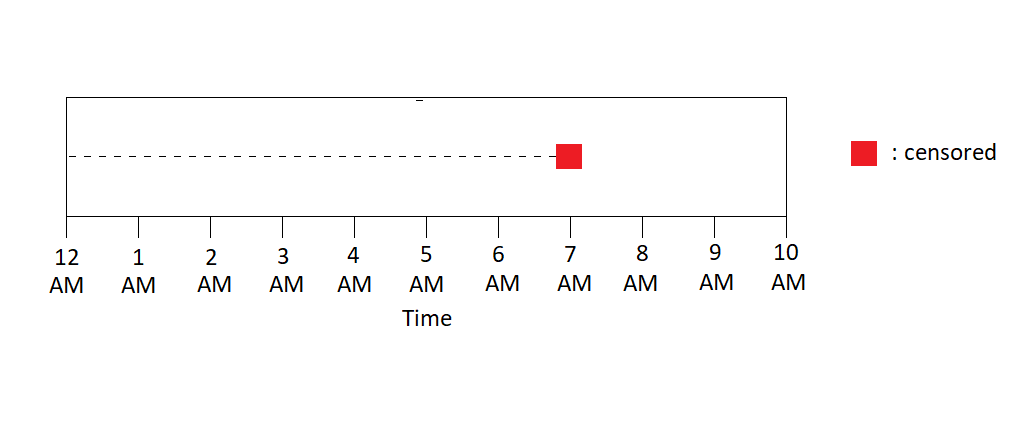
\includegraphics[width=1\linewidth]{figures/left_censoring_example_fix} 

}

\caption{Left Censoring Example}\label{fig:leftcensoringexample}
\end{figure}
Left censoring is a specific instance of censoring in which we only know that the true value of a data point falls below a certain threshold which we call the \emph{limit of detection} (LOD).

To understand this concept better, consider the following example. Imagine a scenario in which you are attempting to estimate the time at which the sun rises each morning. You plan to wake up every morning far before the sun rises, but on the first day of the study, you oversleep and wake up at 7:00 A.M. with the sun already out. We now have an instance of left-censored data. We want to know the time at which the sun rose, but all we have is an upper limit (7:00 A.M.).

Left censoring is commonly found in environmental, water quality, and chemical-related research where the focus is on the concentration of an analyte. Due to limitations on measuring instruments, left censored data are commonly found in these types of studies. The most pressing issue of left-censored data mostly lie in the difficulty of distinguishing between extremely low values and statistical noise (Hall, Perry, \& Anderson, 2020).

\hypertarget{challenges}{%
\section{Challenges of Reporting Censored Data}\label{challenges}}

There is no universal reporting practice for values below the LOD which can lead to confusion amongst researchers. The lack of standardization makes it difficult to distinguish LOD values with uncensored values. This can lead to LOD values unintentionally being overlooked, causing faulty analysis or conclusions which are heavily flawed.

In a study involving the precision of lead measurements near concentrations of the limit of detection, Berthouex (1993) discusses the disparity in practices within chemists on ways to record LOD values. He enumerates in a following list, common reporting practices in this field:
\begin{enumerate}
  \item Reporting the trace, a chemical whose average concentration is less than 100 $\mu g$
  \item Reporting  the letters ND, which stand for "not detected"
  \item Reporting the numerical LOD value itself
  \item Reporting "<", followed by the numerical LOD value
  \item Reporting some value between 0 and the LOD value, such as one-half the LOD value
  \item Reporting the actual measured concentration, even if it falls below the LOD
  \item Reporting the actual measured concentration, followed by "(LOD)"
  \item Reporting the actual measured concentration with a precision ($\pm$) statement
\end{enumerate}
The latter three methods are the best procedures to follow, especially from a practical and statistical point of view according to Gilbert (1987). He argues that assuming the small concentration values are not from some sort of measurement error during data collection, then the value holds value. As such, recording a measurement as ``below LOD,'' without any sort of accompanying value would be discarding useful information which could have been used in practice and analysis.

Berthouex (1993) discusses the prevalence in regards to the practice of censoring data by reporting only values which are above the detection limit and discarding those which fail to yield quantifiable results. He discourages this practice and instead suggests the reporting of measurements, even when those values are below the limit of detection.

Further supporting the stance of keeping all concentration values rather than only those above the detection limit, Monte-Carlo experiements conducted by Gillom (1984) show that linear trends in water-quality data were far more easily able to be detected with uncensored data as compared to censored data. The methods they used to handle censored water quality data were found to produce wild and erratic estimates for the mean and standard deviation of datasets with higher censoring levels than those without. They found a general trend of decreasing classification success with increased censoring levels, attributing it to the limited availability of information in censored data.

\hypertarget{Approaches}{%
\section{Approaches}\label{Approaches}}

It is important to note that the values below the LOD still contain information, specifically that the values is between the lower bound value (if it exists) and the LOD (Chen et al., 2011). As such, there are a variety of statistical treatments to handle censored data which have been popularized in the statistical literature which will be discussed within this section.

Omission involves the deletion of data points which are deemed to be invalid as a result of left-censoring or any other deficiencies in the data. This is also more commonly known as \emph{available-case analysis}, in which statistical analysis is conducted while only considering the observations which have no missing data on the variables of interest, and excluding the observations with missing values (May, 2012). May argues against this approach and claims that the loss of information from discarding data and the inflation of standard errors of estimates (when discussing missingness in a regression context) will invariably be inflated as a result of the decreased sample size. The advantages of omission lies in its ease of implementation.

Apart from available-case analysis, over the past century, a myriad of methods to deal with censoring have been developed to counter this issue -- some more statistically sound than others. We will review some of the most common methods to estimate descriptive statistics involving censored data, which include: substitution, maximum likelihood estimation, Kaplan-Meier, and regression on order statistics (Lafleur et al., 2011).

\hypertarget{Substitution}{%
\subsection{Substitution Method}\label{Substitution}}

Often condemned in papers as a statistically unsound method to handle censored data, substitution methods are ubiquitous in the chemical and environmental sciences as an appropriate and recommended method to work with left-censored chemical concentration data (Canales, 2018).

The substitution method simply involves imputing in a replacement value in lieu of the censored data point. The lack of a global, standardized replacement value to substitute is one of the most pronounced downside of this method. The replacement value used may differ between studies but common values include: \(\frac{LOD}{2}, \frac{LOD}{\sqrt2}\), or \(LOD\) (Lee \& Helsel, 2005). Different disciplines have their own suggested ``best'' replacement value to use, an example being \(\frac{3}{4}\) times the LOD being a common replacement value in geochemistry (Crovelli, 1993). However, it must be recognized that the substitution method is a statistically unsound technique which is often used in non-rigorous statistical settings due to them being quite easy to implement (Chen et al., 2011). As such, there have been several studies in order to investigate the effectiveness of the method.

Proponents of the substitution method claim that the replacement value \(\frac{LOD}{2}\) is useful for data sets in which the majority of the data are below the LOD or when the distribution of the data is highly skewed; the definition of ``highly skewed'' being any distribution with a geometric standard deviation (a measure of spread commonly used in tandem with log-normal distributions) of 3 or more (Hornung \& Reed, 1989). They also suggest using \(\frac{LOD}{\sqrt2}\) when there are only a few data points below the LOD or when the data is not highly skewed.

Substitution methods are flawed as they can often introduce a ``signal'' which was not originally present within the data, or even obstruct an actual signal which was present in the original data (Lee \& Helsel, 2005). Numerous authors have advised against the usage of substitution methods for being statistically inappropriate to use. Glass and Gray (2001) found that both introduce large errors and biases in descriptive statistics of interest. Thompson and Nelson (2001) conducted a study in which they found similar results, in that it often led to biased parameter estimates and ``artificially small standard error estimates.'' Hewett and Ganser (2007) also found in their simulation study that the substitution method yielded the lowest average bias and root mean squared error values (comparison metrics to measure accuracy) in their estimation of the mean. Overall, the overall consensus seems to advise against the practice of these substitution techniques.

{[}paragraph talking about proponents of the substitution methods??{]}

\hypertarget{MLE}{%
\subsection{Maximum Likelihood Estimation Method}\label{MLE}}

Maximum likelihood (ML) estimation is a parametric technique which allows us to estimate the parameters of a distribution or model when the data is from a multivariate normal distribution.

To give a brief introduction to the mechanisms of ML estimation, let \(f(x|\theta)\) denote the probability density function (PDF) which specifies the probability of observing the random variable \(x\) given the parameter \(\theta\).

Given a random, independently and identically distributed (\emph{i.i.d.}) set of random variables \(X_1, X_2,...,X_n\) from \(f(x|\theta)\), we know that each individual observation \(x_i\)'s are statistically independent from one another, which allows us to express the PDF as the product of all individual densities. For every observed random sample \(x_1,...,x_n\), we can define the joint density function to be:

\[f(x_1,...,x_n|\theta) = f(x_1|\theta)...f(x_n|\theta) = \prod_{i=1}^{n}f(x_i|\theta)\]
In most real-life scenarios, the actual (observed) data is already given, and our goal is to find the PDF which is most likely to generate our observed values. In order to solve this inverse problem, we introduce the likelihood function, which is defined as the joint density of the observed data as a function of the parameter (with the data held as a fixed constant).

In mathematical notation, upon observing the given data, \(f(x_1,...,x_n|\Theta)\) becomes a function of \(\theta\) alone, so we obtain a likelihood of:

\[lik(\theta) = f(x_1,...,x_n|\theta)\]
It is important to recognize the difference which separates the likelihood function and the PDF. The PDF is a function of the observed data given a parameter(s). It gives information regarding the probability of a particular data value for a fixed parameter.

On the other hand, the likelihood function is a function of the parameter, given a set of observed data. It tells us the likelihood of observing a particular parameter value for a fixed set of data.

Our goal is to obtain the ML estimate of our parameter which maximizes the likelihood function, \(lik(\theta)\), in other words, to obtain a \(\theta\) which makes our observed data the most probable.

As we previously declared our random variables \(X_1, X_2,...,X_n\) to be i.i.d, we can rewrite the likelihood to be a product of the marginal densities:

\[lik(\theta) = \prod_{i=1}^{n} f(x_i|\theta)\]
in which we can then maximize the likelihood to find the best mle of \(\theta\) to best capture our observed data.

Yavuz et al.~(2017) discuss the usage of MLE method, when missing data is present, and note that it is only appropriate to use for non-negative probability distributions such as: exponential, log-normal, normal, and Weibull.

When left censoring is present, the likelihood function changes in order to account for both the censored observations and the uncensored observations and becomes:

\[lik(\theta) = \prod_{i=1}^n f(x_i|\theta)^{\delta_{i}} \ \times F(x_i|\theta)^{1-{\delta_{i}}}\]

in which \(\delta_{i}\) is an indicator, representing whether or not if the \(i\)th observation is censored or not:

\[\delta_i =
\begin{cases}
  0, & \text{if censored} \\
  1, & \text{if uncensored}
\end{cases}\]
From this updated definition of the likelihood function which must be used in the presence of left censored data, it is then possible to follow typical procedures to find the estimator, \(\theta\), which maximizes the likelihood, also known as the \emph{maximum likelihood estimator}. With this knowledge, the descriptive statistics of interest (mean, variance, etc.) relating to the specified distribution can be calculated.

Canales (2018) outlines a imputation technique which involves replacing censored observations with values from the estimated parameterized distribution. However, is not mentioned explicitly how this imputation method is conducted.

The code for the MLE method will be handled with the \texttt{cenmle} function in the \texttt{NADA} package, which allows the user to specify censored and uncensored data, and uses the LOD as the placeholder. As this method is not an imputation technique, values are not replaced. This method allows us to calculate the summary statistics for the entire data set -- including the censored values. (remove and write own code??)

As a technique which heavily relies upon knowing a distribution which best models the data, MLE is one of the most well-known parametric approaches to handling LOD values. Many studies use the MLE as a sort of baseline method of handling censored values, to which they compare their new techniques upon (Ganser \& Hewett, 2010). However, it must be known that regardless of the prevalence of the MLE method, it is not free from its own downfalls. Canales (2018) found that the MLE method seems to underperform when the data in question was highly skewed, in which overinflated mean squared errors were often obtained. Being a technique which is so heavily dependent upon distributional assumptions, an incorrect specification of the distribution of the censored data will inevitably lead to misleading results (Bolks, DeWire, \& Harcum, 2014).

\hypertarget{rkm}{%
\subsection{Kaplan-Meier Method}\label{rkm}}

As a phenomenon, censoring is most often discussed in survival analysis, which concerns itself with techniques to analyze a time to an \emph{event variable}. As its name suggests, these variables measure the time which passes until some sort of event occurs. This can be as innocuous as the time until device breaks, time until birds migrate away from their homes, time until a person passes away, etc. Regardless of which, all these scenarios share a common problem in terms of the possibility of the data being ``censored.''

The Kaplan-Meier (KM) method is a common nonparametric technique used to deal with censored data. Nonparametric methods do not utilize any information regarding the parameters for a specified distribution, like the mean and standard deviation for the normal distribution. The KM method was originally developed to handle right-censored survival analysis data. The advantages of the KM method lie in its robustness as a nonparametric method, it performs well without having to depend upon distributional assumptions. Many recommend its usage for when there are cases of severe censoring, instances where \textgreater{} 90\% of the data is censored (Canales, 2018).

To introduce the concept of the KM-estimator, it is helpful to take a look into its usages in survival analysis studies where the focus is often on a type of data known as ``time to event'' data. These types of studies often involve events such time to death, time to failure, and so forth.

The KM-estimator is a statistic used to estimate the survival curve from the empirical data while accounting for the possibilities of certain values being censored. It does this by assuming that censoring is independent from the event of interest and that survival probabilities remain the same in observations found early in the study and those recruited later in the study.

The KM-estimator when performing an empirical estimation of the survival curve at time \(t\) can be represented by the following equation:

\[\hat{S}(t) = \prod_{\ t_i \le \ t }\left(1-\frac{d_i}{n_i}\right)\]
where \(t_i\) is the distinct event time, \(d_i\) is the number of event occurrences at time \(t_i\), and \(n_i\) is the number of followup times (\(t_i\)) that are \(\ge\) \(t_i\) (how many observations in sample survived at least/or past the time \(t_i\)) (Klein \& Moeschberge, 2003).

Typically, the KM-estimator can only be used to estimate the distribution function of right-censored data, in which a data point is above a certain threshold, but it is unknown by how much. A simple tweak to the typical KM-method, allows for the estimation of the survival curve with left-censored values.

Helsel (2005, as cited in Yavuz et al., 2017) provides a detailed explanation on how to apply the KM method when left censoring is present. Firstly, it is essential to reverse the left-censored data through a transformation algorithm before using the KM method to change them into right-censored data.

Let \(x_i\) \(\ldots\) \(x_n\) be the values for the observations \(i = 1, 2, ..., n\). Arrange all the left-censored values in descending order and then subtract them by \(M\), a constant bigger than the biggest value of the dataset, in order to get the transformed, right-censored value, \(M-x_i\). All values are then arranged in ascending order to be used to estimate the survival function through the Kaplan-Meier estimator.

It must be known that the KM-method is not an imputation procedure, but instead an estimation technique that allows for the calculation of descriptive statistics for left-censored datasets. Nian (1997 gives the expressions to calculate the estimated mean, median, and variance below:

\(\hat{\mu} = \int_{0}^{\infty} \hat{S}(t) \ dt\)
\(\hat{M} = \hat{S}^{-1} \left (\frac{1}{2} \right)\)
\(Var(\hat{\mu}) = \sum_{i=1}^{r} \left( \int_{t_i}^{\infty}\hat{S}(t) \ dt \right)^2 \frac{d_i}{n_i(n_i - d_i)}\)

\hypertarget{ROS}{%
\subsection{Regression on Order Statistics}\label{ROS}}

Lastly, regression on order statistics (ROS) combines both the parametric nature of the MLE approach and nonparametric nature of the KM method. ROS is a semi-parametric method which assumes an underlying normal or lognormal distribution for the censored measurements but makes no assumption towards the distribution of uncensored measurements.

(Environmental Protection Agency, 2009) provides a a more detailed explanation to the methodology of ROS, but the basic procedures will be outlined in this thesis.

ROS begins with the estimation of the cumulative probability associated with each distinct LOD. This cumulative probability is distributed equally between the censored values with a common LOD (see (Environmental Protection Agency, 2009), for more details). A regression model is fit between the uncensored values and the distributional quantiles. The slope and intercept of the regression line from this model is then used to estimate the mean and standard deviation of the distributional model which are then used to generate imputed values for the censored observations.

In order for ROS to be utilized, there needs to be at least 5 known values and more than half the values within the censored variables must be known. As regression is utilized in this method, the response variable must also be a linear function of the explanatory variable (quantiles). Additionally, the errors should have constant variance (Lee \& Helsel, 2005).

The \texttt{NADA} package contains the function \texttt{ros} which provides an implementation of regression on order statistics which allows us to calculate descriptive statistics for left censored values.

{[}INSERT PARAGRAPH TO TRANSITION TO CHAPTER 3 (?){]}

\hypertarget{simulations}{%
\chapter{Simulations}\label{simulations}}

Having discussed the various methods to handle left-censored data in the previous chapter, we now turn to a simulation study in order to evaluate the strengths and weaknesses of each method in cases of differing censoring rate, sample size, and distribution. We will also discuss the implementation of the methods, data generating mechanisms, and specific evaluation metrics to assess the performance of each method.

\hypertarget{aims}{%
\section{Aims}\label{aims}}

The question of which method is the best to use is frequently discussed topic within the field. Many studies have been conducted over the years to evaluate the performance of these methods to handle left-censored data, with the results being widely varied and largely inconclusive. First and foremost, a large issue comes in that every conducted study widely differs in the methods being investigated and the scope of the study. As an example of the broad differences between studies which can make comparisons difficult, (Antweiler, 2015) evaluates the effectiveness of 11 different methods with several censoring rates and distributional assumptions, using the median absolute deviation (MAD) as their performance metric of choice. Meanwhile, (Hall, Perry, \& Anderson, 2020) focuses instead on the applications of such methods from a water-quality focused context and investigates the performance of the four methods used in this thesis -- except with water stream concentration data, and no focus on distributional assumptions nor censoring rates. As each of these studies are concerned with their own goals -- the reasoning and conclusion that they reach will inevitably be different. Studies that are more focused on a general, broad audience, with no assumptions as to what sort of data the individual is working with -- may find more use with the conclusion and results that investigators like Antweiler come up with. There may also be individuals who are more focused on the performance of such methods in a specific context, as in the study conducted by Hall. There is no common ground between statisticians on the optimality of methods, prompting our own foray into this topic. I wish to incorporate the detailed specifications of a simulation study, while keeping it applicable towards the coal contamination water quality data that I am hoping to apply the methods to.

Through our simulation study, we wish to identify settings where a method can be effective but also those in which the methods may not be able to perform quite as well. Several investigators in this field have found issues with certain methods underperforming under certain conditions, and brings up the possibility of particular methods being more equipped than others to deal with different rates of censoring. Specifically, a study on methodologies to handling left-censored microbial risk assessment conducted by (Canales, 2018) found that the substitution method seemed to work much better than expected while other methods, such as the MLE method, seemed to have trouble when applied to highly skewed data. Results from other works (Antweiler, 2015) suggest that regardless of the method being utilized, obtaining reliable estimates from datasets where censoring was greater than 40\% was unfeasible. This particular study also suggests that the size of the data had no influence on the result of the estimate in question.

Claims regarding the effectiveness of methods with regards to censoring rates, distribution of data, and sample size are all highly contentious. In order to get a better idea of sense of how these claims hold up, our goal is to evaluate the validity of those claims by conducting a simulation study of our own which will put those claims into practice. We must note that we don't expect one method to be significantly above the others in terms of performance for all settings, but we do hope to see which method might be best for certain settings, in terms of distributional assumptions, censoring rates, and sample sizes. This approach and aim of our simulation study will then largely depend on how we will generate the data to be used in order to achieve our goal.

\hypertarget{data_generating_mechanisms}{%
\section{Data-Generating Mechanisms}\label{data_generating_mechanisms}}

The data generated for use in our study will be obtained by using parametric draws from user-specified distributions (log-normal, exponential, and Weibull), as the methods utilized can only be used with non-negative distributions (Yavuz, Tekindal, \& Dog, 2017). Our data-generating mechanism also alters criterion such as the sample size, \(n_{obs} = \{10, 100, 1000\}\) and censoring rate \(R = \{0.10, 0.20, 0.30, 0.40, 0.50\}\).

Censored values are generated and determined by first arranging the uncensored observations in ascending order, and then from the censoring rate. For instance, if our censoring rate were \(R = 0.15\), the lowest 0.15 of the observations will be marked as censored while the rest remain uncensored.

\hypertarget{estimands}{%
\section{Estimands}\label{estimands}}

Each of the four methods discussed in the previous chapter are designed for usage in obtaining summary statistics for left censored data (Shoari, 2018). in our simulation study, we want to evaluate just how well these methods are able to estimate a population quantity. We will be using the sample mean as an estimator for our estimand, the population mean, \(\mu\).

\hypertarget{performance_measures}{%
\section{Performance Measures}\label{performance_measures}}

Morris et al.~(2019) define performance measures as numeric metrics used to assess the performance of the method in question. The criterions we will use to assess the performance of each of our four methods will consist of: bias, variance, and mean squared error (MSE).

\hypertarget{variance}{%
\subsection{Variance}\label{variance}}

Before defining variance, it is important to have a good grasp of the concept of precision. Precision simply refers to how far away estimates from different samples are from one another. Low precision indicates that the estimates from each sample are close to one another in value and vice versa.

Knowing this, variance is a metric which informs us on the precision of an estimator. It is defined as simply the average squared deviation of the estimator from its average, which in our case is defined as:

\(Variance = E[(\hat{\mu}-E(\hat{\mu}))^2]\)

Estimators with low variances generally remain close in value throughout all samples, while those with high variance may wildly differ between samples. As such, it is generally preferable to have an estimator with low variance. However, it is important to note that precision measurements, such as the variance, are not a sole indicator of an estimator's performance (Walther \& Moore, 2005). While precise estimators are ideal, it is also important to assess the estimator's bias, how close it is to the true value.

\hypertarget{bias}{%
\subsection{Bias}\label{bias}}

Bias is defined as the difference between an estimator's expected value and the true value of the parameter. In our case, we are using the estimator \(\hat{\mu}\) to ``estimate'' the true population mean, \(\mu\), in each of our samples. As such, bias can be defined in our case as:

\(Bias = E(\hat{\mu}) - \mu\)

It is important to note that bias is a metric which only informs us on the difference of the estimator from the true parameter, and tells us nothing regarding accuracy nor precision.

If the bias of an estimator were to be equal to zero, we would define the estimator to be \emph{unbiased}, meaning that the estimator produces parameter estimates which are on average, equal to the true value.

However, it is important to note that just because an estimator is unbiased, does not necessarily tell us anything about the quality of our estimator (of being good or bad). An unbiased estimator could have high variance, which would mean that the estimator in each sample would be significantly different from one another, but on average -- they equal the true population estimand.

On that same note, it would not be very useful if an estimator had low variance but high bias, either -- as this would mean that each sample would consistently produce similar estimates which are very far away from the true population estimand in question.

\hypertarget{mean-squared-error-mse}{%
\subsection{Mean Squared Error (MSE)}\label{mean-squared-error-mse}}

We generally would like estimators which have low bias and low variance, but it can be difficult to achieve both at once. As such, it is common to instead turn to a quantity known as the mean squared error (MSE), which is a quantitative measurement used to assess the accuracy of an estimator. The MSE measures how far away, on average, an estimator is from its true value.

(NOTE: section below is VERY messy, need to clean up, play around with math mode, blah)

\(MSE = E[(\hat{\mu} -\mu)^2] = Var(\hat{\mu})+[Bias(\hat{\mu})]^2\)

We can show that the MSE of estimator can be rewritten in terms of its variance and bias:

\[E[(\hat{\mu} -\mu)^2] = E(\hat{\mu}^2) + \mu^2 - 2E(\hat{\mu})\mu\]
Since we know bias to be \(Bias = E(\hat{\mu}) - \mu\), it follows that \(Bias^2 = E^2(\hat{\mu}) +\mu^2 -2E(\hat{\mu})\theta\). We already know variance to be \(Variance = E[(\hat{\mu}-E(\hat{\mu}))^2] = E(\hat{\mu}^2) - E^2(\hat{\mu})\). Thus, combining the square of the bias with variance yields:

\(Bias^2 + Var = [E^2(\hat{\mu}) +\mu^2 -2E(\hat{\mu})\theta] + [E(\hat{\mu}^2) - E^2(\hat{\mu})]\) the \(E^2(\hat{\mu})\) terms cancel out, and we are left with: \(E^2(\hat{\mu}) +\mu^2 -2E(\hat{\mu})\theta = E[(\hat{\mu} -\mu)^2] = Bias\).

As the MSE is always positive, MSE values closer to zero are more desirable -- as it is an indicator that the estimator is accurate.

\hypertarget{results}{%
\section{Results}\label{results}}

{[}place figures/tables from results of simulation study here, along with explanation{]}

The results of our simulation study are presented in the following tables below.
\begin{table}

\caption{\label{tab:unnamed-chunk-1}Performance metrics of our our 
             4 methods with data derived from the log-normal 
             distribution with mean = 1 and SD = 0.5.}
\centering
\fontsize{11.5}{13.5}\selectfont
\begin{tabular}[t]{lrrrrr}
\toprule
  & Sample Size & Avg. Mean & Bias & Variance & MSE\\
\midrule
\addlinespace[0.3em]
\multicolumn{6}{l}{\textbf{Censoring Rate = 0.1}}\\
\hspace{1em}km & 10 & 1.009 & 0.00924 & 0.02289 & 0.02295\\
\hspace{1em}mle & 10 & 0.997 & -0.00262 & 0.02276 & 0.02275\\
\hspace{1em}ros & 10 & 0.991 & -0.00923 & 0.02190 & 0.02197\\
\hspace{1em}substitution & 10 & 0.981 & -0.01901 & 0.02201 & 0.02235\\
\hspace{1em}km & 100 & 1.008 & 0.00766 & 0.00263 & 0.00268\\
\hspace{1em}mle & 100 & 0.998 & -0.00178 & 0.00263 & 0.00263\\
\hspace{1em}ros & 100 & 0.999 & -0.00142 & 0.00258 & 0.00258\\
\hspace{1em}substitution & 100 & 0.983 & -0.01707 & 0.00255 & 0.00284\\
\hspace{1em}km & 1000 & 1.009 & 0.00913 & 0.00024 & 0.00033\\
\hspace{1em}mle & 1000 & 1.000 & -0.00004 & 0.00024 & 0.00024\\
\hspace{1em}ros & 1000 & 1.001 & 0.00127 & 0.00024 & 0.00024\\
\hspace{1em}substitution & 1000 & 0.985 & -0.01536 & 0.00024 & 0.00047\\
\addlinespace[1em]
\multicolumn{6}{l}{\textbf{Censoring Rate = 0.3}}\\
\hspace{1em}km & 10 & 1.050 & 0.05015 & 0.02754 & 0.03002\\
\hspace{1em}mle & 10 & 0.968 & -0.03235 & 0.02431 & 0.02534\\
\hspace{1em}ros & 10 & 0.976 & -0.02381 & 0.02374 & 0.02429\\
\hspace{1em}substitution & 10 & 0.937 & -0.06286 & 0.02298 & 0.02691\\
\hspace{1em}km & 100 & 1.049 & 0.04904 & 0.00288 & 0.00528\\
\hspace{1em}mle & 100 & 0.974 & -0.02628 & 0.00252 & 0.00321\\
\hspace{1em}ros & 100 & 1.000 & -0.00001 & 0.00259 & 0.00259\\
\hspace{1em}substitution & 100 & 0.944 & -0.05642 & 0.00241 & 0.00559\\
\hspace{1em}km & 1000 & 1.049 & 0.04939 & 0.00026 & 0.00270\\
\hspace{1em}mle & 1000 & 0.974 & -0.02554 & 0.00024 & 0.00089\\
\hspace{1em}ros & 1000 & 1.004 & 0.00377 & 0.00024 & 0.00025\\
\hspace{1em}substitution & 1000 & 0.945 & -0.05540 & 0.00022 & 0.00329\\
\addlinespace[1em]
\multicolumn{6}{l}{\textbf{Censoring Rate = 0.5}}\\
\hspace{1em}km & 10 & 1.148 & 0.14806 & 0.03718 & 0.05907\\
\hspace{1em}mle & 10 & 0.908 & -0.09188 & 0.02236 & 0.03078\\
\hspace{1em}ros & 10 & 0.967 & -0.03257 & 0.02810 & 0.02914\\
\hspace{1em}substitution & 10 & 0.908 & -0.09229 & 0.02368 & 0.03217\\
\hspace{1em}km & 100 & 1.129 & 0.12867 & 0.00372 & 0.02027\\
\hspace{1em}mle & 100 & 0.904 & -0.09649 & 0.00240 & 0.01171\\
\hspace{1em}ros & 100 & 0.996 & -0.00399 & 0.00316 & 0.00317\\
\hspace{1em}substitution & 100 & 0.904 & -0.09614 & 0.00250 & 0.01174\\
\hspace{1em}km & 1000 & 1.129 & 0.12885 & 0.00035 & 0.01695\\
\hspace{1em}mle & 1000 & 0.905 & -0.09535 & 0.00023 & 0.00932\\
\hspace{1em}ros & 1000 & 1.005 & 0.00515 & 0.00029 & 0.00032\\
\hspace{1em}substitution & 1000 & 0.905 & -0.09484 & 0.00023 & 0.00923\\
\bottomrule
\end{tabular}
\end{table}
\begin{table}

\caption{\label{tab:unnamed-chunk-2}Performance metrics of our our 3 
             methods (MLE method absent) with data derived from the 
             exponential distribution with a shape parameter = 1.}
\centering
\fontsize{11.5}{13.5}\selectfont
\begin{tabular}[t]{lrrrrr}
\toprule
  & Sample Size & Avg. Mean & Bias & Variance & MSE\\
\midrule
\addlinespace[0.3em]
\multicolumn{6}{l}{\textbf{Censoring Rate = 0.1}}\\
\hspace{1em}km & 10 & 1.012 & 0.01191 & 0.06330 & 0.06341\\
\hspace{1em}mle & 10 &  &  &  \vphantom{2} & \\
\hspace{1em}ros & 10 & 0.997 & -0.00265 & 0.06173 & 0.06170\\
\hspace{1em}substitution & 10 & 0.992 & -0.00761 & 0.06186 & 0.06189\\
\hspace{1em}km & 100 & 1.010 & 0.00974 & 0.00646 & 0.00656\\
\hspace{1em}mle & 100 &  &  &  \vphantom{2} & \\
\hspace{1em}ros & 100 & 1.005 & 0.00469 & 0.00647 & 0.00648\\
\hspace{1em}substitution & 100 & 0.994 & -0.00553 & 0.00649 & 0.00652\\
\hspace{1em}km & 1000 & 1.007 & 0.00693 & 0.00067 & 0.00072\\
\hspace{1em}mle & 1000 &  &  &  \vphantom{2} & \\
\hspace{1em}ros & 1000 & 1.003 & 0.00308 & 0.00066 & 0.00067\\
\hspace{1em}substitution & 1000 & 0.992 & -0.00798 & 0.00071 & 0.00077\\
\addlinespace[1em]
\multicolumn{6}{l}{\textbf{Censoring Rate = 0.3}}\\
\hspace{1em}km & 10 & 1.063 & 0.06291 & 0.07325 & 0.07717\\
\hspace{1em}mle & 10 &  &  &  \vphantom{1} & \\
\hspace{1em}ros & 10 & 0.991 & -0.00916 & 0.06389 & 0.06394\\
\hspace{1em}substitution & 10 & 0.970 & -0.02978 & 0.06372 & 0.06457\\
\hspace{1em}km & 100 & 1.053 & 0.05270 & 0.00719 & 0.00996\\
\hspace{1em}mle & 100 &  &  &  \vphantom{1} & \\
\hspace{1em}ros & 100 & 1.011 & 0.01140 & 0.00685 & 0.00698\\
\hspace{1em}substitution & 100 & 0.972 & -0.02764 & 0.00717 & 0.00793\\
\hspace{1em}km & 1000 & 1.054 & 0.05368 & 0.00073 & 0.00361\\
\hspace{1em}mle & 1000 &  &  &  \vphantom{1} & \\
\hspace{1em}ros & 1000 & 1.017 & 0.01683 & 0.00085 & 0.00113\\
\hspace{1em}substitution & 1000 & 0.974 & -0.02557 & 0.00152 & 0.00217\\
\addlinespace[1em]
\multicolumn{6}{l}{\textbf{Censoring Rate = 0.5}}\\
\hspace{1em}km & 10 & 1.193 & 0.19309 & 0.10925 & 0.14648\\
\hspace{1em}mle & 10 &  &  &  & \\
\hspace{1em}ros & 10 & 0.992 & -0.00789 & 0.07636 & 0.07638\\
\hspace{1em}substitution & 10 & 0.968 & -0.03151 & 0.07419 & 0.07514\\
\hspace{1em}km & 100 & 1.162 & 0.16154 & 0.00992 & 0.03601\\
\hspace{1em}mle & 100 &  &  &  & \\
\hspace{1em}ros & 100 & 1.023 & 0.02269 & 0.00792 & 0.00844\\
\hspace{1em}substitution & 100 & 0.961 & -0.03925 & 0.00946 & 0.01100\\
\hspace{1em}km & 1000 & 1.163 & 0.16301 & 0.00201 & 0.02858\\
\hspace{1em}mle & 1000 &  &  &  & \\
\hspace{1em}ros & 1000 & 1.036 & 0.03598 & 0.00164 & 0.00293\\
\hspace{1em}substitution & 1000 & 0.964 & -0.03594 & 0.00405 & 0.00534\\
\bottomrule
\end{tabular}
\end{table}
\begin{table}

\caption{\label{tab:unnamed-chunk-3}Performance metrics of our our 3 methods 
             (MLE method absent) with data derived from the Weibull 
             distribution with a shape parameter = 1 and 
             scale parameter = 1.}
\centering
\fontsize{11.5}{13.5}\selectfont
\begin{tabular}[t]{lrrrrr}
\toprule
  & Sample Size & Avg. Mean & Bias & Variance & MSE\\
\midrule
\addlinespace[0.3em]
\multicolumn{6}{l}{\textbf{Censoring Rate = 0.1}}\\
\hspace{1em}km & 10 & 1.010 & 0.00977 & 0.07703 & 0.07710\\
\hspace{1em}mle & 10 &  &  &  \vphantom{2} & \\
\hspace{1em}ros & 10 & 0.997 & -0.00339 & 0.07518 & 0.07516\\
\hspace{1em}substitution & 10 & 0.993 & -0.00678 & 0.07525 & 0.07527\\
\hspace{1em}km & 100 & 1.010 & 0.00998 & 0.00768 & 0.00778\\
\hspace{1em}mle & 100 &  &  &  \vphantom{2} & \\
\hspace{1em}ros & 100 & 1.006 & 0.00626 & 0.00768 & 0.00772\\
\hspace{1em}substitution & 100 & 0.998 & -0.00215 & 0.00768 & 0.00768\\
\hspace{1em}km & 1000 & 1.006 & 0.00625 & 0.00077 & 0.00081\\
\hspace{1em}mle & 1000 &  &  &  \vphantom{2} & \\
\hspace{1em}ros & 1000 & 1.004 & 0.00374 & 0.00077 & 0.00079\\
\hspace{1em}substitution & 1000 & 0.995 & -0.00548 & 0.00081 & 0.00084\\
\addlinespace[1em]
\multicolumn{6}{l}{\textbf{Censoring Rate = 0.3}}\\
\hspace{1em}km & 10 & 1.067 & 0.06660 & 0.08638 & 0.09078\\
\hspace{1em}mle & 10 &  &  &  \vphantom{1} & \\
\hspace{1em}ros & 10 & 0.996 & -0.00440 & 0.07540 & 0.07540\\
\hspace{1em}substitution & 10 & 0.981 & -0.01896 & 0.07526 & 0.07559\\
\hspace{1em}km & 100 & 1.054 & 0.05434 & 0.00845 & 0.01140\\
\hspace{1em}mle & 100 &  &  &  \vphantom{1} & \\
\hspace{1em}ros & 100 & 1.016 & 0.01566 & 0.00804 & 0.00829\\
\hspace{1em}substitution & 100 & 0.982 & -0.01761 & 0.00825 & 0.00856\\
\hspace{1em}km & 1000 & 1.055 & 0.05451 & 0.00085 & 0.00382\\
\hspace{1em}mle & 1000 &  &  &  \vphantom{1} & \\
\hspace{1em}ros & 1000 & 1.021 & 0.02059 & 0.00094 & 0.00136\\
\hspace{1em}substitution & 1000 & 0.984 & -0.01618 & 0.00152 & 0.00178\\
\addlinespace[1em]
\multicolumn{6}{l}{\textbf{Censoring Rate = 0.5}}\\
\hspace{1em}km & 10 & 1.221 & 0.22073 & 0.12826 & 0.17694\\
\hspace{1em}mle & 10 &  &  &  & \\
\hspace{1em}ros & 10 & 1.009 & 0.00898 & 0.08864 & 0.08869\\
\hspace{1em}substitution & 10 & 0.998 & -0.00169 & 0.08642 & 0.08639\\
\hspace{1em}km & 100 & 1.173 & 0.17290 & 0.01172 & 0.04162\\
\hspace{1em}mle & 100 &  &  &  & \\
\hspace{1em}ros & 100 & 1.033 & 0.03267 & 0.00934 & 0.01040\\
\hspace{1em}substitution & 100 & 0.980 & -0.01968 & 0.01051 & 0.01090\\
\hspace{1em}km & 1000 & 1.173 & 0.17294 & 0.00201 & 0.03192\\
\hspace{1em}mle & 1000 &  &  &  & \\
\hspace{1em}ros & 1000 & 1.045 & 0.04497 & 0.00165 & 0.00367\\
\hspace{1em}substitution & 1000 & 0.982 & -0.01751 & 0.00372 & 0.00402\\
\bottomrule
\end{tabular}
\end{table}
From the results of our simulation study, we can see that with the data generated from the log-normal distribution, in the case of low censoring (0.10), when dealing with sample sizes of 10 and 100, the methods are largely comparable to one another. Substitution and KM do not perform quite as well as ROS and MLE, both displaying an increase in absolute bias and MSE when compared to the latter two. Substitution performs significant worse than KM. MLE and ROS perform rather equally well in all sample sizes for low-censoring.

When considering medium censoring (0.30), much of the same observations still hold true. Substitution performs the worse, followed by KM. MLE and ROS both perform well. However, ROS has a slight edge over MLE, especially as sample sizes increase, attaining lower MSE values than the latter.

All four methods begin to perform worse when the censoring rate is increased to 0.5, which is to be expected. As more and more missingness is introduced within the dataset, it becomes more difficult to obtain accurate estimates for all methods. Once again, substitution and KM attain high absolute bias and MSE values. However, it is now KM which performs worse than substitution in the setting of high censoring. Similarly to before, albeit being more noticeable now, ROS performs better than MLE with all sample sizes.

We can see with the exponential and Weibull cases, all three methods perform equally well in the case of low (0.10) censoring with all sample sizes, obtaining similar bias and MSE values across all sample sizes for both the exponential and Weibull datasets. KM consistently performs the worst with with medium (0.30) and high (0.50) censoring when compared to the other methods across all sample sizes. In these censoring settings, it is also the case that ROS performs the best with substitution not far behind.

In summary, regardless of distributional assumptions all of the methods perform well when censoring is low, with very minute differences in performance metrics. KM does not perform well in the lognormal distribution with high censoring rates and struggles in the exponential and Weibull cases with medium and high censoring rates. While MLE was only used in the case of the lognormal data, it also performs quite well, although not quite as well as ROS. ROS performed the best in the case of medium and high censoring across all 3 distributions.

\hypertarget{discussion}{%
\section{Discussion}\label{discussion}}

It important to note that while there are a large number of papers which discuss the ideal method or strategy to handle left-censored data,these studies have a large number of differences in censoring rates, distribution used, methods used, and other aspects of design setups which make comparisons regarding the results obtained from the studies quite difficult. As such, descriptions of specifics regarding the study design in the following studies will be omitted as necessary.

Several results from our simulation studies agree with previous findings conducted from other investigators in the field. Gilliom \& Helsel (1986) claims that with the lognormal distribution, the ROS method was superior. This claim is furthered with our own results: we find that the ROS method is rather robust, even with censoring and produces an accurate and precise estimate of the mean in all cases in our simulation study.

Another investigation by Kroll \& Stedinger (1996) found that with regards to a lognormal distribution only, ROS and MLE worked extremely well, with MLE outperforming the other methods especially in highly censored cases. While the MLE method did perform rather well in most cases in our simulation study, it did not outperform the ROS method, which in fact obtained much better estimates of the mean in highly censored settings.

There are of course also studies which offer differing results from the ones we obtained in our simulation study.

Schmoyer, Beauchamp, Brandt, \& Hoffman (1996) compared only MLE and KM and found that the KM method performed nearly as well as the MLE in the case of the lognormal distribution. However, this was not the case in our simulation study. While the KM and MLE methods were able to perform adequately in the case of low (0.1) and medium (0.3) censoring, they performed the worst out of all four methods when dealing with highly censored cases. The censoring rates used in their study consisted of 25\%, 50\%, and 70\% -- which far exceeded the censoring values used in this thesis.

She (1997) conducted a study investigating censored water quality data with the intent of investigating how well the KM method performs with regards to the same methods we utilize in this thesis. The results from She's study showed that KM outperformed all other methods, which contradicts the findings in the simulation study conducted in this thesis. Upon further investigation, the size of the dataset utilized by She consisted of 56 observations from water monitoring stations, in which around 11 were censored (20\% of the dataset). While the KM method is not ideal for highly censored cases from the results of our simulation study, it certainly is able to be used for smaller sample sizes -- which is further supported with She's findings. There may be a difference in how well the methods perform with actual data as compared to simulated data -- which we will investigate in the next chapter.

\hypertarget{limitations}{%
\subsection{Limitations}\label{limitations}}

Shortcomings in the results presented in this study may come from the fact that we generated data with known distributional parameters. It could be the case that the effectiveness of our methods were only due to having such artificial data. Alterations in our study to instead generate data from methods such as randomized pulls from an a real-world dataset of interest via. methods such as bootstrapping could provide different insights. As we discussed previously with the results from She (1997), methods may perform differently when utilized with artificial datasets as compared to real world, left censored data. We do not claim our findings in the simulation study to be representative for all cases of left censored data.

\hypertarget{real_data}{%
\section{Study on Real Data}\label{real_data}}

{[}can write this chapter after some preliminary exploration with coal groundwater data{]}

\hypertarget{casestudy}{%
\chapter{Case Study}\label{casestudy}}

\hypertarget{background}{%
\section{Background}\label{background}}

Coal is one of the most prevalent combustible fuels being burned all across the world, as it is one of the easiest methods of obtaining energy due to the abundance of the substance. Generally, coal plants produce electricity by burning coal, which produces coal ash as a byproduct. Over 100 million tons of coal ash are produced every year at these plants, which are then disposed through landfills and waste ponds at these plants. The main concern of ecologists regarding this matter is that the coal ash produced by these plants can often contaminate the local groundwater, leading to toxic contaminants being found in local water sources. Coal ash is dangerous due to its composition, which contains a long list of dangerous chemicals including -- but not limited to: arsenic, radium, boron, and a large list of other contaminants toxic to humans and animals alike (Kelderman et al., 2019).

Complaints and concerns regarding the disposing practices of coal plants have only increased after the 2010 Kingston Fossil Plant coal ash incident in Tennessee. This area has become an attractive location in which many sites of ecological studies have been conducted the years following the incident. Leaching experiments conducted by Ruhl, Vengosh, Dwyer, Hsu-Kim, \& Deonarine (2010) has revealed significant levels of dissolved Arsenic, Boron, Strontium, and Barium in the water which has been in contact with the coal ash, which they note to be threat to infaunal species in the water. Prompted by environmental organizations, groups, and individuals alike, an onslaught of pressure was put on the Environmental Protection Agency, which resulted in the Coal Ash Rule being put into effect in 2015 (Kelderman et al., 2019).

This rule has forced over 265 coal power plants -- about 3/4 of all coal power plants in the US - to make data regarding chemical concentrations publicly available to the general population. In their analysis using this data, the Environmental Integrity Project (2020) -- a non-profit organization dedicated to issues involving environmental justice, has discussed the prevalence of groundwater contamination for wells located near coal related facilities.
\begin{figure}

{\centering 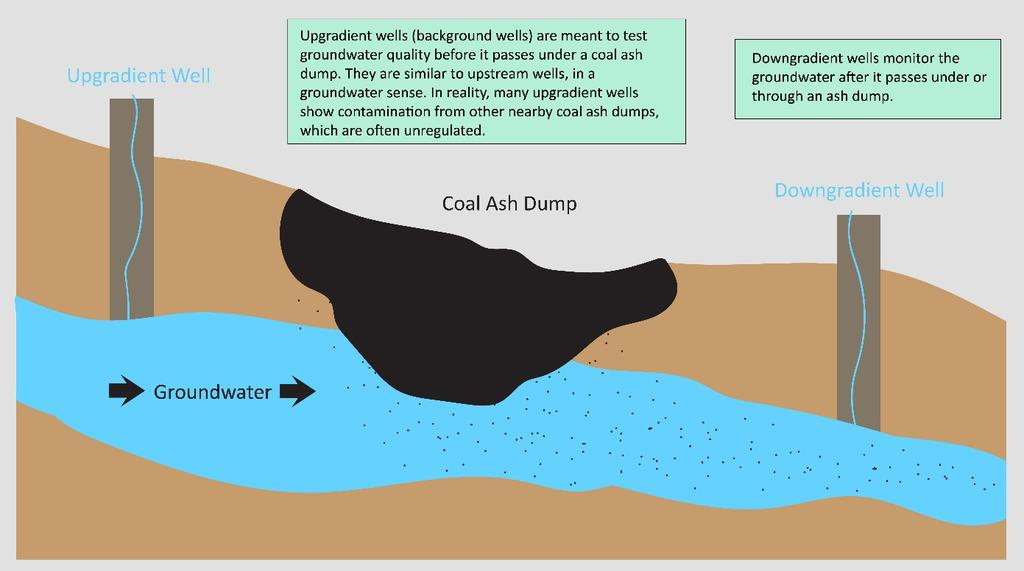
\includegraphics[width=1\linewidth]{figures/upgradientdowngradient} 

}

\caption{Difference Between Upgradient and Downgradient Wells}\label{fig:upgradientdowngradient}
\end{figure}
Typically in a coal ash plant, there exists two types of wells: upgradient wells and downgradient wells. These wells are essential to measure the amount of contamination being caused by coal ash. Upgradient wells, also known as background wells, measures the concentrations of chemicals in groundwater before it passes through an coal ash dump. Conversely, downgradient wells measure the concentrations of chemicals in groundwater after it passes through a coal ash dump.

While both types of well are susceptible to contamination through coal ash related means, it is more frequently the case that we focus on the downgradient wells, as they are more closely linked to the water accessed by the general public.

The goal of the study conducted by Kelderman et al. (2019) was to identify the percentage of coal plants which have unsafe levels of contamination. Determining whether if a well was contaminated or not was largely influenced by the average mean concentrations of the contaminant in question for that well. If the average mean contamination of a contaminant, say, arsenic, was above the health-based threshold considered necessary to ensure safety, then that well would be marked as an ``exceedance,'' and deemed to be contaminated.

Kelderman et al. (2019) notes the possibility of contamination being caused by an external factor, unrelated to the coal ash, and provides a stipulation as how to account for this. They excluded tallying the wells in which the mean downgradient values were lower than the mean upgradient values, as this would mean that the contamination was not caused by the coal plant itself.

Our end goal remains the same as the Kelderman et al. (2019): to identify contaminated groundwater in coal plants. In their report, it is not mentioned if left censored values were being accounted for in the calculations of the average concentrations of the downgradient and upgradient wells. As such, it may be prudent to check to see if the proportion of wells in the U.S. in which contamination is present would be altered if we used our techniques to calculate the average concentrations of the contaminants.

The limit of detection problem stems from the measuring devices' inability to obtain chemical concentrations smaller than a certain threshold amount, thus affecting the measurements recorded.

\hypertarget{data}{%
\section{Data}\label{data}}

It is important to note where the data used originated from, before we delve into the details of our case study. As such, a brief history regarding the Coal Ash Rule and its origin will be explored, alongside details regarding our coal ash dataset.

\hypertarget{coalashrule}{%
\subsection{Coal Ash Rule}\label{coalashrule}}

A large coal ash spill at the Tennessee Valley Authority (TVA) which occurred on December 22, 2008 in Kingston, TN -- prompted the Environmental Protection Agency (EPA) to propose a set of standardized regulations and procedures to address the concerns regarding coal ash plants nationwide in the US. This was known as the Coal Ash Rule, which passed legislation on December 19, 2014 (Environmental Protection Agency, 2020).

Changes were made to the Coal Ash Rule over the years in the form of `amendments,' in which the most relevant to this study, required coal facilities to publish information and data regarding the concentrations of contaminants in the wells.

\hypertarget{source-of-data}{%
\subsection{Source of Data}\label{source-of-data}}

The data used in the study are from the results published in ``Annual Groundwater Monitoring and Corrective Action Reports,'' which were made available to the public in March 2018 as a result of the Coal Ash Rule. These reports are in PDF format and are thousands of pages long, which makes it difficult for individuals to parse through data in a meaningful way.

The Environmental Integrity Project (2020) obtained the data from an online, publicly available database containing groundwater monitoring results from the first ``Annual Groundwater Monitoring and Corrective Action Reports'' in 2018 which was collected from coal plants and coal ash dumps under the Coal Ash Rule.

They wrangled the data into a more accessible machine-readable format which contains information from over 443 annual groundwater monitoring reports posted by 265 coal ash plants, downloadable from the EIP's website, which we use in our case study.

\newpage

\hypertarget{variables}{%
\subsection{Variables}\label{variables}}

Specifics regarding the variables in the coal dataset can be viewed in Table 3.1. Each observation in the dataset represents a well which measures the concentration of the contaminant in question. Most of the variables are explanatory, such as the state, site, and disposal area in which the well is located in. However, there are several variables specific to groundwater data collection which are important to note.

There are four different types that each well can be classified as, which is represented in the \texttt{type} variable. These consist of: \texttt{L}, \texttt{M}, \texttt{SI}, and \texttt{U} which stand for ``landfill,'' ``mixed,'' ``surface-impacted,'' and "uniform

The coal dataset contains information regarding chemical concentrations at coal plants. A coal plant consists of multiple disposal areas for the coal ash that it produces. At each disposal area, there are specific locations that groundwater is being measured, known as wells, which represent an observation in the dataset.
\begin{table}

\caption{\label{tab:unnamed-chunk-6}Data dictionary for the coal dataset.}
\centering
\begin{tabular}[t]{ll>{\raggedright\arraybackslash}p{7.6cm}}
\toprule
Variable & Variable Name & Description\\
\midrule
State & state & The state where the site is located.\\
\addlinespace
Site & site & The name of the site as it is presented in its
             groundwater monitoring \vphantom{1} report.\\
\addlinespace
Disposal Area & disposal.area & The name of the disposal area(s) as they are presented 
             in the groundwater monitoring report. Note: some wells 
             monitor groundwater from more than one disposal unit.\\
\addlinespace
Type of Well & type & The type of disposal unit. SI = surface impoundment, 
             L= landfill, M = mixed multi-unit (landfill and surface 
             impoundment), and U = unknown.\\
\addlinespace
ID of Well & well.id & The identifier given to each monitoring well in the 
             groundwater monitoring report.\\
\addlinespace
Gradient Type & gradient & The location of the groundwater monitoring well 
             relative to the regulated ash disposal unit it 
             monitors.\\
\addlinespace
Sample Date & samp.date & The date the well was sampled.\\
\addlinespace
Contaminant Name & contaminant & The contaminant name. These have been standardized to 
             allow for analyses across plants.\\
\addlinespace
Measurement Unit & measurement.unit & The concentration units. These include mg/l, ug/l, 
             pCi/l, and standard units (SU) for pH.\\
\addlinespace
Below Detection & below.detection & LOD status for the concentration, '<' indicates that 
             the concentration was below the LOD.\\
\addlinespace
Concentration & concentration & Concentration of contaminant\\
\bottomrule
\end{tabular}
\end{table}
\hypertarget{plan-of-action}{%
\subsection{Plan of Action}\label{plan-of-action}}

The investigation conducted by Kelderman et al. (2019) mentions certain restrictions within the data that we believe may have caused their analysis to potentially be inaccurate. Specifically with the limit of detection problem arises when measuring devices used to measure chemical concentrations are unable to detect below a certain threshold, causing large numbers of observations to be considered ``below detection.'' These values are often encoded as NA or even mistakenly marked as 0. There are no mentions of any attempts to account for or handle these missing values, which is the motivation for this case study.

Our investigation works with methods on handling this missing data through the techniques detailed in chapter 1 in order to obtain more accurate and precise estimates of the mean concentrations of contaminants at coal ash sites. Through our newly obtained estimates, we hope to see if they might lead us to different beliefs than the claims made by Kelderman et al. (2019) regarding the most contaminated wells in the U.S.

\hypertarget{application}{%
\section{Application}\label{application}}

\hypertarget{conclusion}{%
\chapter{Conclusion}\label{conclusion}}

{[}write a few paragraphs to wrap up entire thesis{]}

\appendix

\hypertarget{main-appendix}{%
\chapter{Main Appendix}\label{main-appendix}}

This first appendix includes all of the R chunks of code that were hidden throughout the document (using the \texttt{include\ =\ FALSE} chunk tag) to help with readibility and/or setup.

\hypertarget{in-the-main-file-refref-labels}{%
\section{In the main file \ref{ref-labels}:}\label{in-the-main-file-refref-labels}}

\hypertarget{in-chapter-refref-labels}{%
\section{In Chapter \ref{ref-labels}:}\label{in-chapter-refref-labels}}

\hypertarget{simulation-appendix}{%
\chapter{Simulation Appendix}\label{simulation-appendix}}

The second appendix, Appendix B, contains all necessary code required to run the simulation study.

\hypertarget{libraries}{%
\section{Libraries}\label{libraries}}
\begin{Shaded}
\begin{Highlighting}[]
\FunctionTok{library}\NormalTok{(tidyverse)}
\FunctionTok{library}\NormalTok{(Metrics) }\CommentTok{\#package to help calculate mse}
\FunctionTok{library}\NormalTok{(NADA) }\CommentTok{\#package with implementation of many methods}
\FunctionTok{library}\NormalTok{(survival)}
\FunctionTok{library}\NormalTok{(kableExtra)}
\end{Highlighting}
\end{Shaded}
\hypertarget{generating-data}{%
\section{Generating Data}\label{generating-data}}
\begin{Shaded}
\begin{Highlighting}[]
\CommentTok{\#function will generate a vector of numbers from the lognormal }
\CommentTok{\#distribution and censor them at the given rate}
\CommentTok{\#function will take in arguments for 1) samplesize, 2) logmean, 3)logsd}
\CommentTok{\#4) censoring rate}

\NormalTok{generateLN }\OtherTok{\textless{}{-}} \ControlFlowTok{function}\NormalTok{(sampsize, m, s, censrate)\{}
\NormalTok{  true.value }\OtherTok{\textless{}{-}} \FunctionTok{rlnorm}\NormalTok{(sampsize, }
               \AttributeTok{meanlog=}\FunctionTok{log}\NormalTok{(m}\SpecialCharTok{\^{}}\DecValTok{2} \SpecialCharTok{/} \FunctionTok{sqrt}\NormalTok{(s}\SpecialCharTok{\^{}}\DecValTok{2} \SpecialCharTok{+}\NormalTok{ m}\SpecialCharTok{\^{}}\DecValTok{2}\NormalTok{)),}
               \AttributeTok{sdlog=}\FunctionTok{sqrt}\NormalTok{(}\FunctionTok{log}\NormalTok{(}\DecValTok{1} \SpecialCharTok{+}\NormalTok{ (s}\SpecialCharTok{\^{}}\DecValTok{2} \SpecialCharTok{/}\NormalTok{ m}\SpecialCharTok{\^{}}\DecValTok{2}\NormalTok{))))}
  
\NormalTok{  uncensored\_df }\OtherTok{\textless{}{-}} \FunctionTok{as.data.frame}\NormalTok{(true.value) }\SpecialCharTok{\%\textgreater{}\%}
    \FunctionTok{arrange}\NormalTok{(true.value)}
  
\NormalTok{  censored\_df }\OtherTok{\textless{}{-}}\NormalTok{ uncensored\_df }\SpecialCharTok{\%\textgreater{}\%} \CommentTok{\#take the head(\%) of data to be censored}
    \FunctionTok{slice\_head}\NormalTok{(}\AttributeTok{n=}\FunctionTok{nrow}\NormalTok{(uncensored\_df)}\SpecialCharTok{*}\NormalTok{censrate) }\SpecialCharTok{\%\textgreater{}\%}
    \FunctionTok{mutate}\NormalTok{(}\AttributeTok{censored =} \ConstantTok{TRUE}\NormalTok{)}
  
  \CommentTok{\#full join original df and sliced df}
\NormalTok{  return\_df }\OtherTok{\textless{}{-}} \FunctionTok{full\_join}\NormalTok{(uncensored\_df, censored\_df, }\AttributeTok{by =} \StringTok{"true.value"}\NormalTok{)}

  \CommentTok{\#replace NAs with FALSE}
\NormalTok{  return\_df}\SpecialCharTok{$}\NormalTok{censored }\OtherTok{\textless{}{-}} \FunctionTok{replace\_na}\NormalTok{(return\_df}\SpecialCharTok{$}\NormalTok{censored, }\AttributeTok{replace =} \ConstantTok{FALSE}\NormalTok{)}
  
  \FunctionTok{return}\NormalTok{(return\_df)}
\NormalTok{\}}
\CommentTok{\#function will generate a vector of numbers from the exponential }
\CommentTok{\#distribution and censor them at the given rate}
\CommentTok{\#function will take in arguments for 1) samplesize, 2) rate,}
\CommentTok{\#3) censoring rate}

\NormalTok{generateEXP }\OtherTok{\textless{}{-}} \ControlFlowTok{function}\NormalTok{(sampsize, r, censrate)\{}
\NormalTok{  true.value }\OtherTok{\textless{}{-}} \FunctionTok{rexp}\NormalTok{(sampsize, }\AttributeTok{rate =}\NormalTok{ r)}
  
\NormalTok{  uncensored\_df }\OtherTok{\textless{}{-}} \FunctionTok{as.data.frame}\NormalTok{(true.value) }\SpecialCharTok{\%\textgreater{}\%}
    \FunctionTok{arrange}\NormalTok{(true.value)}
  
\NormalTok{  censored\_df }\OtherTok{\textless{}{-}}\NormalTok{ uncensored\_df }\SpecialCharTok{\%\textgreater{}\%} \CommentTok{\#take the head(\%) of data to be censored}
    \FunctionTok{slice\_head}\NormalTok{(}\AttributeTok{n=}\FunctionTok{nrow}\NormalTok{(uncensored\_df)}\SpecialCharTok{*}\NormalTok{censrate) }\SpecialCharTok{\%\textgreater{}\%}
    \FunctionTok{mutate}\NormalTok{(}\AttributeTok{censored =} \ConstantTok{TRUE}\NormalTok{)}
  
  \CommentTok{\#full join original df and sliced df}
\NormalTok{  return\_df }\OtherTok{\textless{}{-}} \FunctionTok{full\_join}\NormalTok{(uncensored\_df, censored\_df, }\AttributeTok{by =} \StringTok{"true.value"}\NormalTok{)}

  \CommentTok{\#replace NAs with FALSE}
\NormalTok{  return\_df}\SpecialCharTok{$}\NormalTok{censored }\OtherTok{\textless{}{-}} \FunctionTok{replace\_na}\NormalTok{(return\_df}\SpecialCharTok{$}\NormalTok{censored, }\AttributeTok{replace =} \ConstantTok{FALSE}\NormalTok{)}
  
  \FunctionTok{return}\NormalTok{(return\_df)}
\NormalTok{\}}
\CommentTok{\#function will generate a vector of numbers from the Weibull}
\CommentTok{\#distribution and censor them at the given rate}
\CommentTok{\#function will take in arguments for 1) samplesize, 2) rate,}
\CommentTok{\#3) censoring rate}

\NormalTok{generateW }\OtherTok{\textless{}{-}} \ControlFlowTok{function}\NormalTok{(sampsize, sh, sc, censrate)\{}
\NormalTok{  true.value }\OtherTok{\textless{}{-}} \FunctionTok{rweibull}\NormalTok{(sampsize, }\AttributeTok{shape =}\NormalTok{ sh, }\AttributeTok{scale =}\NormalTok{ sc)}
  
\NormalTok{  uncensored\_df }\OtherTok{\textless{}{-}} \FunctionTok{as.data.frame}\NormalTok{(true.value) }\SpecialCharTok{\%\textgreater{}\%}
    \FunctionTok{arrange}\NormalTok{(true.value)}
  
\NormalTok{  censored\_df }\OtherTok{\textless{}{-}}\NormalTok{ uncensored\_df }\SpecialCharTok{\%\textgreater{}\%} \CommentTok{\#take the head(\%) of data to be censored}
    \FunctionTok{slice\_head}\NormalTok{(}\AttributeTok{n=}\FunctionTok{nrow}\NormalTok{(uncensored\_df)}\SpecialCharTok{*}\NormalTok{censrate) }\SpecialCharTok{\%\textgreater{}\%}
    \FunctionTok{mutate}\NormalTok{(}\AttributeTok{censored =} \ConstantTok{TRUE}\NormalTok{)}
  
  \CommentTok{\#full join original df and sliced df}
\NormalTok{  return\_df }\OtherTok{\textless{}{-}} \FunctionTok{full\_join}\NormalTok{(uncensored\_df, censored\_df, }\AttributeTok{by =} \StringTok{"true.value"}\NormalTok{)}

  \CommentTok{\#replace NAs with FALSE}
\NormalTok{  return\_df}\SpecialCharTok{$}\NormalTok{censored }\OtherTok{\textless{}{-}} \FunctionTok{replace\_na}\NormalTok{(return\_df}\SpecialCharTok{$}\NormalTok{censored, }\AttributeTok{replace =} \ConstantTok{FALSE}\NormalTok{)}
  
  \FunctionTok{return}\NormalTok{(return\_df)}
\NormalTok{\}}
\end{Highlighting}
\end{Shaded}
\hypertarget{setup}{%
\section{Setup}\label{setup}}
\begin{Shaded}
\begin{Highlighting}[]
\NormalTok{iterations }\OtherTok{\textless{}{-}} \DecValTok{1000} \CommentTok{\#number of iterations}
\NormalTok{censvalues }\OtherTok{\textless{}{-}} \FunctionTok{c}\NormalTok{(}\FloatTok{0.10}\NormalTok{, }\FloatTok{0.30}\NormalTok{, }\FloatTok{0.50}\NormalTok{)}
\NormalTok{sampsizes }\OtherTok{\textless{}{-}} \FunctionTok{c}\NormalTok{(}\DecValTok{10}\NormalTok{, }\DecValTok{100}\NormalTok{, }\DecValTok{1000}\NormalTok{)}

\NormalTok{df.tall }\OtherTok{\textless{}{-}} \FunctionTok{data.frame}\NormalTok{(}\AttributeTok{prop\_cens =} \FunctionTok{numeric}\NormalTok{(),}
                      \AttributeTok{samplesize =} \FunctionTok{numeric}\NormalTok{(),}
                      \AttributeTok{iteration =} \FunctionTok{numeric}\NormalTok{(),}
                      \AttributeTok{method =} \FunctionTok{character}\NormalTok{(),}
                      \AttributeTok{true\_mean =} \FunctionTok{numeric}\NormalTok{(),}
                      \AttributeTok{mean\_complete =} \FunctionTok{numeric}\NormalTok{(),}
                      \AttributeTok{mean\_method =} \FunctionTok{numeric}\NormalTok{(),}
                      \AttributeTok{true\_sd =} \FunctionTok{numeric}\NormalTok{(),}
                      \AttributeTok{SE\_complete =} \FunctionTok{numeric}\NormalTok{(),}
                      \AttributeTok{SE\_method =} \FunctionTok{numeric}\NormalTok{())}
\end{Highlighting}
\end{Shaded}
\hypertarget{lognormal}{%
\section{Lognormal}\label{lognormal}}
\begin{Shaded}
\begin{Highlighting}[]
\CommentTok{\#LOGNORMAL}
\FunctionTok{options}\NormalTok{(}\AttributeTok{scipen=}\DecValTok{999}\NormalTok{) }\CommentTok{\#prevent scientific notation}
\FunctionTok{set.seed}\NormalTok{(}\DecValTok{7271999}\NormalTok{)}

\ControlFlowTok{for}\NormalTok{(i }\ControlFlowTok{in}\NormalTok{ censvalues)\{}
  \ControlFlowTok{for}\NormalTok{(j }\ControlFlowTok{in}\NormalTok{ sampsizes)\{}
    \ControlFlowTok{for}\NormalTok{(k }\ControlFlowTok{in} \DecValTok{1}\SpecialCharTok{:}\NormalTok{iterations)\{}
\NormalTok{      m }\OtherTok{\textless{}{-}} \DecValTok{1}
\NormalTok{      s }\OtherTok{\textless{}{-}} \FloatTok{0.5}
\NormalTok{      df }\OtherTok{\textless{}{-}} \FunctionTok{generateLN}\NormalTok{(}\AttributeTok{sampsize =}\NormalTok{ j, }\AttributeTok{m =} \DecValTok{1}\NormalTok{, }\AttributeTok{s =} \FloatTok{0.5}\NormalTok{, }\AttributeTok{censrate =}\NormalTok{ i)}
      
      \CommentTok{\#substitution}
      \CommentTok{\#define LOD to be smallest, uncensored value}
\NormalTok{      LOD }\OtherTok{\textless{}{-}} \FunctionTok{min}\NormalTok{(df}\SpecialCharTok{$}\NormalTok{true.value[df}\SpecialCharTok{$}\NormalTok{censored }\SpecialCharTok{==} \ConstantTok{FALSE}\NormalTok{]) }
\NormalTok{      df }\OtherTok{\textless{}{-}}\NormalTok{ df }\SpecialCharTok{\%\textgreater{}\%}
        \FunctionTok{mutate}\NormalTok{(}\AttributeTok{impSubValue =} \FunctionTok{if\_else}\NormalTok{(censored }\SpecialCharTok{==} \ConstantTok{TRUE}\NormalTok{, LOD}\SpecialCharTok{/}\DecValTok{2}\NormalTok{, true.value))}
      
\NormalTok{      df.tall }\OtherTok{\textless{}{-}}\NormalTok{ df.tall }\SpecialCharTok{\%\textgreater{}\%}
        \FunctionTok{add\_row}\NormalTok{(}\AttributeTok{prop\_cens =}\NormalTok{ i,}
                \AttributeTok{samplesize =}\NormalTok{ j,}
                \AttributeTok{iteration =}\NormalTok{ k,}
                \AttributeTok{method =} \StringTok{"substitution"}\NormalTok{,}
                \AttributeTok{true\_mean =}\NormalTok{ m,}
                \AttributeTok{mean\_complete =} \FunctionTok{mean}\NormalTok{(df}\SpecialCharTok{$}\NormalTok{true.value),}
                \AttributeTok{mean\_method =} \FunctionTok{mean}\NormalTok{(df}\SpecialCharTok{$}\NormalTok{impSubValue),}
                \AttributeTok{true\_sd =}\NormalTok{ s,}
                \AttributeTok{SE\_complete =} 
                  \FunctionTok{sd}\NormalTok{(df}\SpecialCharTok{$}\NormalTok{true.value)}\SpecialCharTok{/}\FunctionTok{sqrt}\NormalTok{((}\FunctionTok{length}\NormalTok{(df}\SpecialCharTok{$}\NormalTok{true.value))),}
                \AttributeTok{SE\_method =} 
                  \FunctionTok{sd}\NormalTok{(df}\SpecialCharTok{$}\NormalTok{impSubValue)}\SpecialCharTok{/}\FunctionTok{sqrt}\NormalTok{((}\FunctionTok{length}\NormalTok{(df}\SpecialCharTok{$}\NormalTok{impSubValue))))}
      
      \CommentTok{\#mle}
\NormalTok{      mle\_res }\OtherTok{=} \FunctionTok{cenmle}\NormalTok{(df}\SpecialCharTok{$}\NormalTok{true.value, df}\SpecialCharTok{$}\NormalTok{censored)}
      
\NormalTok{      df.tall }\OtherTok{\textless{}{-}}\NormalTok{ df.tall }\SpecialCharTok{\%\textgreater{}\%}
        \FunctionTok{add\_row}\NormalTok{(}\AttributeTok{prop\_cens =}\NormalTok{ i,}
                \AttributeTok{samplesize =}\NormalTok{ j,}
                \AttributeTok{iteration =}\NormalTok{ k,}
                \AttributeTok{method =} \StringTok{"mle"}\NormalTok{,}
                \AttributeTok{true\_mean =}\NormalTok{ m,}
                \AttributeTok{mean\_complete =} \FunctionTok{mean}\NormalTok{(df}\SpecialCharTok{$}\NormalTok{true.value),}
                \AttributeTok{mean\_method =} \FunctionTok{mean}\NormalTok{(mle\_res)[}\DecValTok{1}\NormalTok{],}
                \AttributeTok{true\_sd =}\NormalTok{ s,}
                \AttributeTok{SE\_complete =} 
                  \FunctionTok{sd}\NormalTok{(df}\SpecialCharTok{$}\NormalTok{true.value)}\SpecialCharTok{/}\FunctionTok{sqrt}\NormalTok{((}\FunctionTok{length}\NormalTok{(df}\SpecialCharTok{$}\NormalTok{true.value))),}
                \AttributeTok{SE\_method =} \FunctionTok{mean}\NormalTok{(mle\_res)[}\DecValTok{2}\NormalTok{])}
      
      \CommentTok{\#km}
\NormalTok{      km\_res }\OtherTok{=} \FunctionTok{cenfit}\NormalTok{(df}\SpecialCharTok{$}\NormalTok{true.value, df}\SpecialCharTok{$}\NormalTok{censored)}
      
\NormalTok{      df.tall }\OtherTok{\textless{}{-}}\NormalTok{ df.tall }\SpecialCharTok{\%\textgreater{}\%}
        \FunctionTok{add\_row}\NormalTok{(}\AttributeTok{prop\_cens =}\NormalTok{ i,}
                \AttributeTok{samplesize =}\NormalTok{ j,}
                \AttributeTok{iteration =}\NormalTok{ k,}
                \AttributeTok{method =} \StringTok{"km"}\NormalTok{,}
                \AttributeTok{true\_mean =}\NormalTok{ m,}
                \AttributeTok{mean\_complete =} \FunctionTok{mean}\NormalTok{(df}\SpecialCharTok{$}\NormalTok{true.value),}
                \AttributeTok{mean\_method =} \FunctionTok{mean}\NormalTok{(km\_res)[[}\DecValTok{1}\NormalTok{]],}
                \AttributeTok{true\_sd =}\NormalTok{ s,}
                \AttributeTok{SE\_complete =} 
                  \FunctionTok{sd}\NormalTok{(df}\SpecialCharTok{$}\NormalTok{true.value)}\SpecialCharTok{/}\FunctionTok{sqrt}\NormalTok{((}\FunctionTok{length}\NormalTok{(df}\SpecialCharTok{$}\NormalTok{true.value))),}
                \AttributeTok{SE\_method =} \FunctionTok{mean}\NormalTok{(km\_res)[[}\DecValTok{2}\NormalTok{]])}
      
      \CommentTok{\#ros}
\NormalTok{      ros\_res }\OtherTok{=} \FunctionTok{ros}\NormalTok{(df}\SpecialCharTok{$}\NormalTok{true.value, df}\SpecialCharTok{$}\NormalTok{censored)}
      
\NormalTok{      df.tall }\OtherTok{\textless{}{-}}\NormalTok{ df.tall }\SpecialCharTok{\%\textgreater{}\%}
        \FunctionTok{add\_row}\NormalTok{(}\AttributeTok{prop\_cens =}\NormalTok{ i,}
                \AttributeTok{samplesize =}\NormalTok{ j,}
                \AttributeTok{iteration =}\NormalTok{ k,}
                \AttributeTok{method =} \StringTok{"ros"}\NormalTok{,}
                \AttributeTok{true\_mean =}\NormalTok{ m,}
                \AttributeTok{mean\_complete =} \FunctionTok{mean}\NormalTok{(df}\SpecialCharTok{$}\NormalTok{true.value),}
                \AttributeTok{mean\_method =} \FunctionTok{mean}\NormalTok{(ros\_res),}
                \AttributeTok{true\_sd =}\NormalTok{ s,}
                \AttributeTok{SE\_complete =} 
                  \FunctionTok{sd}\NormalTok{(df}\SpecialCharTok{$}\NormalTok{true.value)}\SpecialCharTok{/}\FunctionTok{sqrt}\NormalTok{((}\FunctionTok{length}\NormalTok{(df}\SpecialCharTok{$}\NormalTok{true.value))),}
                \AttributeTok{SE\_method =} 
                  \FunctionTok{sd}\NormalTok{(ros\_res)}\SpecialCharTok{/}\FunctionTok{sqrt}\NormalTok{((}\FunctionTok{length}\NormalTok{(df}\SpecialCharTok{$}\NormalTok{true.value))))}
\NormalTok{    \}}
    \CommentTok{\#end of \# iterations}
\NormalTok{  \}}
\NormalTok{\}}

\CommentTok{\#aggregating performance criteria}

\NormalTok{df.ln }\OtherTok{\textless{}{-}}\NormalTok{ df.tall }\SpecialCharTok{\%\textgreater{}\%}
  \FunctionTok{group\_by}\NormalTok{(prop\_cens, samplesize, method) }\SpecialCharTok{\%\textgreater{}\%}
  \FunctionTok{summarize}\NormalTok{(}\AttributeTok{Avg\_Mean =} \FunctionTok{mean}\NormalTok{(mean\_method),}
            \AttributeTok{Bias =}\NormalTok{ (}\FunctionTok{mean}\NormalTok{(mean\_method) }\SpecialCharTok{{-}}\NormalTok{ true\_mean),}
            \AttributeTok{Variance =} \FunctionTok{var}\NormalTok{(mean\_method),}
            \AttributeTok{MSE =} \FunctionTok{mse}\NormalTok{(true\_mean, mean\_method) }
\NormalTok{            ) }\SpecialCharTok{\%\textgreater{}\%}
  \FunctionTok{distinct}\NormalTok{() }\SpecialCharTok{\%\textgreater{}\%}
  \FunctionTok{ungroup}\NormalTok{()}
\end{Highlighting}
\end{Shaded}
\hypertarget{exponential}{%
\section{Exponential}\label{exponential}}
\begin{Shaded}
\begin{Highlighting}[]
\CommentTok{\#EXPONENTIAL}
\FunctionTok{options}\NormalTok{(}\AttributeTok{scipen=}\DecValTok{999}\NormalTok{) }\CommentTok{\#prevent scientific notation}
\FunctionTok{set.seed}\NormalTok{(}\DecValTok{7271999}\NormalTok{)}

\ControlFlowTok{for}\NormalTok{(i }\ControlFlowTok{in}\NormalTok{ censvalues)\{}
  \ControlFlowTok{for}\NormalTok{(j }\ControlFlowTok{in}\NormalTok{ sampsizes)\{}
    \ControlFlowTok{for}\NormalTok{(k }\ControlFlowTok{in} \DecValTok{1}\SpecialCharTok{:}\NormalTok{iterations)\{}
\NormalTok{      r }\OtherTok{=} \DecValTok{1}
\NormalTok{      df }\OtherTok{\textless{}{-}} \FunctionTok{generateEXP}\NormalTok{(}\AttributeTok{sampsize =}\NormalTok{ j, }\AttributeTok{r =}\NormalTok{ r, }\AttributeTok{censrate =}\NormalTok{ i)}

      \CommentTok{\#substitution}
      \CommentTok{\#define LOD to be smallest, uncensored value}
\NormalTok{      LOD }\OtherTok{\textless{}{-}} \FunctionTok{min}\NormalTok{(df}\SpecialCharTok{$}\NormalTok{true.value[df}\SpecialCharTok{$}\NormalTok{censored }\SpecialCharTok{==} \ConstantTok{FALSE}\NormalTok{]) }
\NormalTok{      df }\OtherTok{\textless{}{-}}\NormalTok{ df }\SpecialCharTok{\%\textgreater{}\%}
        \FunctionTok{mutate}\NormalTok{(}\AttributeTok{impSubValue =} \FunctionTok{if\_else}\NormalTok{(censored }\SpecialCharTok{==} \ConstantTok{TRUE}\NormalTok{, LOD}\SpecialCharTok{/}\DecValTok{2}\NormalTok{, true.value))}
      
\NormalTok{      df.tall }\OtherTok{\textless{}{-}}\NormalTok{ df.tall }\SpecialCharTok{\%\textgreater{}\%}
        \FunctionTok{add\_row}\NormalTok{(}\AttributeTok{prop\_cens =}\NormalTok{ i,}
                \AttributeTok{samplesize =}\NormalTok{ j,}
                \AttributeTok{iteration =}\NormalTok{ k,}
                \AttributeTok{method =} \StringTok{"substitution"}\NormalTok{,}
                \AttributeTok{true\_mean =} \DecValTok{1}\SpecialCharTok{/}\NormalTok{r,}
                \AttributeTok{mean\_complete =} \FunctionTok{mean}\NormalTok{(df}\SpecialCharTok{$}\NormalTok{true.value),}
                \AttributeTok{mean\_method =} \FunctionTok{mean}\NormalTok{(df}\SpecialCharTok{$}\NormalTok{impSubValue),}
                \AttributeTok{true\_sd =} \DecValTok{1}\SpecialCharTok{/}\NormalTok{r,}
                \AttributeTok{SE\_complete =} 
                  \FunctionTok{sd}\NormalTok{(df}\SpecialCharTok{$}\NormalTok{true.value)}\SpecialCharTok{/}\FunctionTok{sqrt}\NormalTok{((}\FunctionTok{length}\NormalTok{(df}\SpecialCharTok{$}\NormalTok{true.value))),}
                \AttributeTok{SE\_method =} 
                  \FunctionTok{sd}\NormalTok{(df}\SpecialCharTok{$}\NormalTok{impSubValue)}\SpecialCharTok{/}\FunctionTok{sqrt}\NormalTok{((}\FunctionTok{length}\NormalTok{(df}\SpecialCharTok{$}\NormalTok{impSubValue))))}
      
      \CommentTok{\#mle}
      \CommentTok{\# mle\_res = cenmle(df$true.value, df$censored)}
      \CommentTok{\# }
      \CommentTok{\# df.tall \textless{}{-} df.tall \%\textgreater{}\%}
      \CommentTok{\#   add\_row(prop\_cens = i,}
      \CommentTok{\#           samplesize = j,}
      \CommentTok{\#           iteration = k,}
      \CommentTok{\#           method = "mle",}
      \CommentTok{\#           true\_mean = 1/r,}
      \CommentTok{\#           mean\_complete = mean(df$true.value),}
      \CommentTok{\#           mean\_method = mean(mle\_res)[1],}
      \CommentTok{\#           true\_sd = 1/r,}
      \CommentTok{\#           SE\_complete = }
      \CommentTok{\#             sd(df$true.value)/sqrt((length(df$true.value))),}
      \CommentTok{\#           SE\_method = mean(mle\_res)[2])}
      
\NormalTok{      df.tall }\OtherTok{\textless{}{-}}\NormalTok{ df.tall }\SpecialCharTok{\%\textgreater{}\%}
        \FunctionTok{add\_row}\NormalTok{(}\AttributeTok{prop\_cens =}\NormalTok{ i,}
                \AttributeTok{samplesize =}\NormalTok{ j,}
                \AttributeTok{iteration =}\NormalTok{ k,}
                \AttributeTok{method =} \StringTok{"mle"}\NormalTok{,}
                \AttributeTok{true\_mean =} \ConstantTok{NA}\NormalTok{,}
                \AttributeTok{mean\_complete =} \ConstantTok{NA}\NormalTok{,}
                \AttributeTok{mean\_method =} \ConstantTok{NA}\NormalTok{,}
                \AttributeTok{true\_sd =} \ConstantTok{NA}\NormalTok{,}
                \AttributeTok{SE\_complete =} \ConstantTok{NA}\NormalTok{,}
                \AttributeTok{SE\_method =} \ConstantTok{NA}\NormalTok{)}
      
      \CommentTok{\#km}
\NormalTok{      km\_res }\OtherTok{=} \FunctionTok{cenfit}\NormalTok{(df}\SpecialCharTok{$}\NormalTok{true.value, df}\SpecialCharTok{$}\NormalTok{censored)}
      
\NormalTok{      df.tall }\OtherTok{\textless{}{-}}\NormalTok{ df.tall }\SpecialCharTok{\%\textgreater{}\%}
        \FunctionTok{add\_row}\NormalTok{(}\AttributeTok{prop\_cens =}\NormalTok{ i,}
                \AttributeTok{samplesize =}\NormalTok{ j,}
                \AttributeTok{iteration =}\NormalTok{ k,}
                \AttributeTok{method =} \StringTok{"km"}\NormalTok{,}
                \AttributeTok{true\_mean =} \DecValTok{1}\SpecialCharTok{/}\NormalTok{r,}
                \AttributeTok{mean\_complete =} \FunctionTok{mean}\NormalTok{(df}\SpecialCharTok{$}\NormalTok{true.value),}
                \AttributeTok{mean\_method =} \FunctionTok{mean}\NormalTok{(km\_res)[[}\DecValTok{1}\NormalTok{]],}
                \AttributeTok{true\_sd =} \DecValTok{1}\SpecialCharTok{/}\NormalTok{r,}
                \AttributeTok{SE\_complete =} 
                  \FunctionTok{sd}\NormalTok{(df}\SpecialCharTok{$}\NormalTok{true.value)}\SpecialCharTok{/}\FunctionTok{sqrt}\NormalTok{((}\FunctionTok{length}\NormalTok{(df}\SpecialCharTok{$}\NormalTok{true.value))),}
                \AttributeTok{SE\_method =} \FunctionTok{mean}\NormalTok{(km\_res)[[}\DecValTok{2}\NormalTok{]])}
      
      \CommentTok{\#ros}
\NormalTok{      ros\_res }\OtherTok{=} \FunctionTok{ros}\NormalTok{(df}\SpecialCharTok{$}\NormalTok{true.value, df}\SpecialCharTok{$}\NormalTok{censored)}
      
\NormalTok{      df.tall }\OtherTok{\textless{}{-}}\NormalTok{ df.tall }\SpecialCharTok{\%\textgreater{}\%}
        \FunctionTok{add\_row}\NormalTok{(}\AttributeTok{prop\_cens =}\NormalTok{ i,}
                \AttributeTok{samplesize =}\NormalTok{ j,}
                \AttributeTok{iteration =}\NormalTok{ k,}
                \AttributeTok{method =} \StringTok{"ros"}\NormalTok{,}
                \AttributeTok{true\_mean =} \DecValTok{1}\SpecialCharTok{/}\NormalTok{r,}
                \AttributeTok{mean\_complete =} \FunctionTok{mean}\NormalTok{(df}\SpecialCharTok{$}\NormalTok{true.value),}
                \AttributeTok{mean\_method =} \FunctionTok{mean}\NormalTok{(ros\_res),}
                \AttributeTok{true\_sd =} \DecValTok{1}\SpecialCharTok{/}\NormalTok{r,}
                \AttributeTok{SE\_complete =} 
                  \FunctionTok{sd}\NormalTok{(df}\SpecialCharTok{$}\NormalTok{true.value)}\SpecialCharTok{/}\FunctionTok{sqrt}\NormalTok{((}\FunctionTok{length}\NormalTok{(df}\SpecialCharTok{$}\NormalTok{true.value))),}
                \AttributeTok{SE\_method =} 
                  \FunctionTok{sd}\NormalTok{(ros\_res)}\SpecialCharTok{/}\FunctionTok{sqrt}\NormalTok{((}\FunctionTok{length}\NormalTok{(df}\SpecialCharTok{$}\NormalTok{true.value))))}
\NormalTok{    \}}
    \CommentTok{\#end of \# iterations}
\NormalTok{  \}}
\NormalTok{\}}

\CommentTok{\#aggregating performance criteria}

\NormalTok{df.exp }\OtherTok{\textless{}{-}}\NormalTok{ df.tall }\SpecialCharTok{\%\textgreater{}\%}
  \FunctionTok{group\_by}\NormalTok{(prop\_cens, samplesize, method) }\SpecialCharTok{\%\textgreater{}\%}
  \FunctionTok{summarize}\NormalTok{(}\AttributeTok{Avg\_Mean =} \FunctionTok{mean}\NormalTok{(mean\_method),}
            \AttributeTok{Bias =}\NormalTok{ (}\FunctionTok{mean}\NormalTok{(mean\_method) }\SpecialCharTok{{-}}\NormalTok{ true\_mean),}
            \AttributeTok{Variance =} \FunctionTok{var}\NormalTok{(mean\_method),}
            \AttributeTok{MSE =} \FunctionTok{mse}\NormalTok{(true\_mean, mean\_method) }
\NormalTok{            ) }\SpecialCharTok{\%\textgreater{}\%}
  \FunctionTok{distinct}\NormalTok{() }\SpecialCharTok{\%\textgreater{}\%}
  \FunctionTok{ungroup}\NormalTok{()}
\end{Highlighting}
\end{Shaded}
\hypertarget{weibull}{%
\section{Weibull}\label{weibull}}
\begin{Shaded}
\begin{Highlighting}[]
\CommentTok{\#WEIBULL}
\FunctionTok{options}\NormalTok{(}\AttributeTok{scipen=}\DecValTok{999}\NormalTok{) }\CommentTok{\#prevent scientific notation}
\FunctionTok{set.seed}\NormalTok{(}\DecValTok{7271999}\NormalTok{)}

\ControlFlowTok{for}\NormalTok{(i }\ControlFlowTok{in}\NormalTok{ censvalues)\{}
  \ControlFlowTok{for}\NormalTok{(j }\ControlFlowTok{in}\NormalTok{ sampsizes)\{}
    \ControlFlowTok{for}\NormalTok{(k }\ControlFlowTok{in} \DecValTok{1}\SpecialCharTok{:}\NormalTok{iterations)\{}
\NormalTok{      sh }\OtherTok{=} \DecValTok{1}
\NormalTok{      sc }\OtherTok{=} \DecValTok{1}
\NormalTok{      df }\OtherTok{\textless{}{-}} \FunctionTok{generateW}\NormalTok{(}\AttributeTok{sampsize =}\NormalTok{ j, }\AttributeTok{sh =}\NormalTok{ sh, }\AttributeTok{sc =}\NormalTok{ sc, }\AttributeTok{censrate =}\NormalTok{ i)}

      \CommentTok{\#substitution}
      \CommentTok{\#define LOD to be smallest, uncensored value}
\NormalTok{      LOD }\OtherTok{\textless{}{-}} \FunctionTok{min}\NormalTok{(df}\SpecialCharTok{$}\NormalTok{true.value[df}\SpecialCharTok{$}\NormalTok{censored }\SpecialCharTok{==} \ConstantTok{FALSE}\NormalTok{]) }
\NormalTok{      df }\OtherTok{\textless{}{-}}\NormalTok{ df }\SpecialCharTok{\%\textgreater{}\%}
        \FunctionTok{mutate}\NormalTok{(}\AttributeTok{impSubValue =} \FunctionTok{if\_else}\NormalTok{(censored }\SpecialCharTok{==} \ConstantTok{TRUE}\NormalTok{, LOD}\SpecialCharTok{/}\DecValTok{2}\NormalTok{, true.value))}
      
\NormalTok{      df.tall }\OtherTok{\textless{}{-}}\NormalTok{ df.tall }\SpecialCharTok{\%\textgreater{}\%}
        \FunctionTok{add\_row}\NormalTok{(}\AttributeTok{prop\_cens =}\NormalTok{ i,}
                \AttributeTok{samplesize =}\NormalTok{ j,}
                \AttributeTok{iteration =}\NormalTok{ k,}
                \AttributeTok{method =} \StringTok{"substitution"}\NormalTok{,}
                \AttributeTok{true\_mean =}\NormalTok{ sc}\SpecialCharTok{*}\FunctionTok{gamma}\NormalTok{(}\DecValTok{1}\SpecialCharTok{+}\NormalTok{(}\DecValTok{1}\SpecialCharTok{/}\NormalTok{sh)),}
                \AttributeTok{mean\_complete =} \FunctionTok{mean}\NormalTok{(df}\SpecialCharTok{$}\NormalTok{true.value),}
                \AttributeTok{mean\_method =} \FunctionTok{mean}\NormalTok{(df}\SpecialCharTok{$}\NormalTok{impSubValue),}
                \AttributeTok{true\_sd =} \FunctionTok{sqrt}\NormalTok{((sc}\SpecialCharTok{\^{}}\DecValTok{2}\NormalTok{)}\SpecialCharTok{*}\NormalTok{(}\FunctionTok{gamma}\NormalTok{(}\DecValTok{1}\SpecialCharTok{+}\NormalTok{(}\DecValTok{2}\SpecialCharTok{/}\NormalTok{sh)) }\SpecialCharTok{{-}} 
\NormalTok{                                      (}\FunctionTok{gamma}\NormalTok{(}\DecValTok{1}\SpecialCharTok{+}\NormalTok{(}\DecValTok{1}\SpecialCharTok{/}\NormalTok{sh)))}\SpecialCharTok{\^{}}\DecValTok{2}\NormalTok{)),}
                \AttributeTok{SE\_complete =} 
                  \FunctionTok{sd}\NormalTok{(df}\SpecialCharTok{$}\NormalTok{true.value)}\SpecialCharTok{/}\FunctionTok{sqrt}\NormalTok{((}\FunctionTok{length}\NormalTok{(df}\SpecialCharTok{$}\NormalTok{true.value))),}
                \AttributeTok{SE\_method =} 
                  \FunctionTok{sd}\NormalTok{(df}\SpecialCharTok{$}\NormalTok{impSubValue)}\SpecialCharTok{/}\FunctionTok{sqrt}\NormalTok{((}\FunctionTok{length}\NormalTok{(df}\SpecialCharTok{$}\NormalTok{impSubValue))))}
      
      \CommentTok{\#mle}
      \CommentTok{\# mle\_res = cenmle(df$true.value, df$censored)}
      \CommentTok{\# }
      \CommentTok{\# df.tall \textless{}{-} df.tall \%\textgreater{}\%}
      \CommentTok{\#   add\_row(prop\_cens = i,}
      \CommentTok{\#           samplesize = j,}
      \CommentTok{\#           iteration = k,}
      \CommentTok{\#           method = "mle",}
      \CommentTok{\#           true\_mean = 1/r,}
      \CommentTok{\#           mean\_complete = mean(df$true.value),}
      \CommentTok{\#           mean\_method = mean(mle\_res)[1],}
      \CommentTok{\#           true\_sd = 1/r,}
      \CommentTok{\#           SE\_complete = }
      \CommentTok{\#             sd(df$true.value)/sqrt((length(df$true.value))),}
      \CommentTok{\#           SE\_method = mean(mle\_res)[2])}
      
\NormalTok{      df.tall }\OtherTok{\textless{}{-}}\NormalTok{ df.tall }\SpecialCharTok{\%\textgreater{}\%}
        \FunctionTok{add\_row}\NormalTok{(}\AttributeTok{prop\_cens =}\NormalTok{ i,}
                \AttributeTok{samplesize =}\NormalTok{ j,}
                \AttributeTok{iteration =}\NormalTok{ k,}
                \AttributeTok{method =} \StringTok{"mle"}\NormalTok{,}
                \AttributeTok{true\_mean =} \ConstantTok{NA}\NormalTok{,}
                \AttributeTok{mean\_complete =} \ConstantTok{NA}\NormalTok{,}
                \AttributeTok{mean\_method =} \ConstantTok{NA}\NormalTok{,}
                \AttributeTok{true\_sd =} \ConstantTok{NA}\NormalTok{,}
                \AttributeTok{SE\_complete =} \ConstantTok{NA}\NormalTok{,}
                \AttributeTok{SE\_method =} \ConstantTok{NA}\NormalTok{)}
      
      \CommentTok{\#km}
\NormalTok{      km\_res }\OtherTok{=} \FunctionTok{cenfit}\NormalTok{(df}\SpecialCharTok{$}\NormalTok{true.value, df}\SpecialCharTok{$}\NormalTok{censored)}
      
\NormalTok{      df.tall }\OtherTok{\textless{}{-}}\NormalTok{ df.tall }\SpecialCharTok{\%\textgreater{}\%}
        \FunctionTok{add\_row}\NormalTok{(}\AttributeTok{prop\_cens =}\NormalTok{ i,}
                \AttributeTok{samplesize =}\NormalTok{ j,}
                \AttributeTok{iteration =}\NormalTok{ k,}
                \AttributeTok{method =} \StringTok{"km"}\NormalTok{,}
                \AttributeTok{true\_mean =}\NormalTok{ sc}\SpecialCharTok{*}\FunctionTok{gamma}\NormalTok{(}\DecValTok{1}\SpecialCharTok{+}\NormalTok{(}\DecValTok{1}\SpecialCharTok{/}\NormalTok{sh)),}
                \AttributeTok{mean\_complete =} \FunctionTok{mean}\NormalTok{(df}\SpecialCharTok{$}\NormalTok{true.value),}
                \AttributeTok{mean\_method =} \FunctionTok{mean}\NormalTok{(km\_res)[[}\DecValTok{1}\NormalTok{]],}
                \AttributeTok{true\_sd =} \FunctionTok{sqrt}\NormalTok{((sc}\SpecialCharTok{\^{}}\DecValTok{2}\NormalTok{)}\SpecialCharTok{*}\NormalTok{(}\FunctionTok{gamma}\NormalTok{(}\DecValTok{1}\SpecialCharTok{+}\NormalTok{(}\DecValTok{2}\SpecialCharTok{/}\NormalTok{sh)) }\SpecialCharTok{{-}} 
\NormalTok{                                      (}\FunctionTok{gamma}\NormalTok{(}\DecValTok{1}\SpecialCharTok{+}\NormalTok{(}\DecValTok{1}\SpecialCharTok{/}\NormalTok{sh)))}\SpecialCharTok{\^{}}\DecValTok{2}\NormalTok{)),}
                \AttributeTok{SE\_complete =} 
                  \FunctionTok{sd}\NormalTok{(df}\SpecialCharTok{$}\NormalTok{true.value)}\SpecialCharTok{/}\FunctionTok{sqrt}\NormalTok{((}\FunctionTok{length}\NormalTok{(df}\SpecialCharTok{$}\NormalTok{true.value))),}
                \AttributeTok{SE\_method =} \FunctionTok{mean}\NormalTok{(km\_res)[[}\DecValTok{2}\NormalTok{]])}
      
      \CommentTok{\#ros}
\NormalTok{      ros\_res }\OtherTok{=} \FunctionTok{ros}\NormalTok{(df}\SpecialCharTok{$}\NormalTok{true.value, df}\SpecialCharTok{$}\NormalTok{censored)}
      
\NormalTok{      df.tall }\OtherTok{\textless{}{-}}\NormalTok{ df.tall }\SpecialCharTok{\%\textgreater{}\%}
        \FunctionTok{add\_row}\NormalTok{(}\AttributeTok{prop\_cens =}\NormalTok{ i,}
                \AttributeTok{samplesize =}\NormalTok{ j,}
                \AttributeTok{iteration =}\NormalTok{ k,}
                \AttributeTok{method =} \StringTok{"ros"}\NormalTok{,}
                \AttributeTok{true\_mean =}\NormalTok{ sc}\SpecialCharTok{*}\FunctionTok{gamma}\NormalTok{(}\DecValTok{1}\SpecialCharTok{+}\NormalTok{(}\DecValTok{1}\SpecialCharTok{/}\NormalTok{sh)),}
                \AttributeTok{mean\_complete =} \FunctionTok{mean}\NormalTok{(df}\SpecialCharTok{$}\NormalTok{true.value),}
                \AttributeTok{mean\_method =} \FunctionTok{mean}\NormalTok{(ros\_res),}
                \AttributeTok{true\_sd =} \FunctionTok{sqrt}\NormalTok{((sc}\SpecialCharTok{\^{}}\DecValTok{2}\NormalTok{)}\SpecialCharTok{*}\NormalTok{(}\FunctionTok{gamma}\NormalTok{(}\DecValTok{1}\SpecialCharTok{+}\NormalTok{(}\DecValTok{2}\SpecialCharTok{/}\NormalTok{sh)) }\SpecialCharTok{{-}} 
\NormalTok{                                      (}\FunctionTok{gamma}\NormalTok{(}\DecValTok{1}\SpecialCharTok{+}\NormalTok{(}\DecValTok{1}\SpecialCharTok{/}\NormalTok{sh)))}\SpecialCharTok{\^{}}\DecValTok{2}\NormalTok{)),}
                \AttributeTok{SE\_complete =} 
                  \FunctionTok{sd}\NormalTok{(df}\SpecialCharTok{$}\NormalTok{true.value)}\SpecialCharTok{/}\FunctionTok{sqrt}\NormalTok{((}\FunctionTok{length}\NormalTok{(df}\SpecialCharTok{$}\NormalTok{true.value))),}
                \AttributeTok{SE\_method =} 
                  \FunctionTok{sd}\NormalTok{(ros\_res)}\SpecialCharTok{/}\FunctionTok{sqrt}\NormalTok{((}\FunctionTok{length}\NormalTok{(df}\SpecialCharTok{$}\NormalTok{true.value))))}
\NormalTok{    \}}
    \CommentTok{\#end of \# iterations}
\NormalTok{  \}}
\NormalTok{\}}

\CommentTok{\#aggregating performance criteria}

\NormalTok{df.w }\OtherTok{\textless{}{-}}\NormalTok{ df.tall }\SpecialCharTok{\%\textgreater{}\%}
  \FunctionTok{group\_by}\NormalTok{(prop\_cens, samplesize, method) }\SpecialCharTok{\%\textgreater{}\%}
  \FunctionTok{summarize}\NormalTok{(}\AttributeTok{Avg\_Mean =} \FunctionTok{mean}\NormalTok{(mean\_method),}
            \AttributeTok{Bias =}\NormalTok{ (}\FunctionTok{mean}\NormalTok{(mean\_method) }\SpecialCharTok{{-}}\NormalTok{ true\_mean),}
            \AttributeTok{Variance =} \FunctionTok{var}\NormalTok{(mean\_method),}
            \AttributeTok{MSE =} \FunctionTok{mse}\NormalTok{(true\_mean, mean\_method) }
\NormalTok{            ) }\SpecialCharTok{\%\textgreater{}\%}
  \FunctionTok{distinct}\NormalTok{() }\SpecialCharTok{\%\textgreater{}\%}
  \FunctionTok{ungroup}\NormalTok{()}
\end{Highlighting}
\end{Shaded}
\hypertarget{corrections}{%
\chapter*{Corrections}\label{corrections}}
\addcontentsline{toc}{chapter}{Corrections}

A list of corrections after submission to department.

Corrections may be made to the body of the thesis, but every such correction will be acknowledged in a list under the heading ``Corrections,'' along with the statement ``When originally submitted, this honors thesis contained some errors which have been corrected in the current version. Here is a list of the errors that were corrected.'' This list will be given on a sheet or sheets to be appended to the thesis. Corrections to spelling, grammar, or typography may be acknowledged by a general statement such as ``30 spellings were corrected in various places in the thesis, and the notation for definite integral was changed in approximately 10 places.'' However, any correction that affects the meaning of a sentence or paragraph should be described in careful detail. The files samplethesis.tex and samplethesis.pdf show what the ``Corrections'' section should look like. Questions about what should appear in the ``Corrections'' should be directed to the Chair.

\backmatter

\hypertarget{references}{%
\chapter*{References}\label{references}}
\addcontentsline{toc}{chapter}{References}

\noindent

\setlength{\parindent}{-0.20in}
\setlength{\leftskip}{0.20in}
\setlength{\parskip}{8pt}

\hypertarget{refs}{}
\begin{CSLReferences}{1}{0}
\leavevmode\hypertarget{ref-Antweiler2015}{}%
Antweiler, R. C. (2015). {Evaluation of Statistical Treatments of Left-Censored Environmental Data Using Coincident Uncensored Data Sets. II. Group Comparisons}. http://doi.org/\href{https://doi.org/10.1021/acs.est.5b02385}{10.1021/acs.est.5b02385}

\leavevmode\hypertarget{ref-Bolks2014}{}%
Bolks, A., DeWire, A., \& Harcum, J. B. (2014). {Baseline Assessment of Left-Censored Environmental Data Using R}. \emph{Technotes}, \emph{9}(2), 153--172. Retrieved from \url{https://www.epa.gov/sites/production/files/2016-05/documents/tech_notes_10_jun2014_r.pdf}

\leavevmode\hypertarget{ref-Canales2018}{}%
Canales, R. (2018). {Methods for Handling Left-Censored Data in Quantitative Microbial Risk Assessment}, \emph{84}(20), 1--10.

\leavevmode\hypertarget{ref-Chen2011}{}%
Chen, H., Quandt, S. A., Grzywacz, J. G., Arcury, T. A., Environmental, S., Perspectives, H., \ldots{} Arcury, T. A. (2011). {A Distribution-Based Multiple Imputation Method for Handling Bivariate Pesticide Data with Values below the Limit of Detection}, \emph{119}(3), 351--356. http://doi.org/\href{https://doi.org/10.1289/ehp.l002124}{10.1289/ehp.l002124}

\leavevmode\hypertarget{ref-Crovelli1993}{}%
Crovelli, R. A. (1993). {An Objective Replacement Method for Censored Geochemical Data}, \emph{25}(1), 59--80.

\leavevmode\hypertarget{ref-EIP2020}{}%
Environmental Integrity Project. (2020). {Coal Ash Groundwater Contamination: Documenting Coal Ash Pollution}. Retrieved from \url{https://environmentalintegrity.org/coal-ash-groundwater-contamination/}

\leavevmode\hypertarget{ref-EPA2009}{}%
Environmental Protection Agency. (2009). \emph{{STATISTICAL ANALYSIS OF GROUNDWATER MONITORING DATA AT RCRA FACILITIES UNIFIED GUIDANCE}}.

\leavevmode\hypertarget{ref-Car2020}{}%
Environmental Protection Agency. (2020). {Disposal of Coal Combustion Residuals from Electric Utilities Rulemakings}. Retrieved from \url{https://www.epa.gov/coalash/coal-ash-rule}

\leavevmode\hypertarget{ref-Ganser2010}{}%
Ganser, G. H., \& Hewett, P. (2010). {An Accurate Substitution Method for Analyzing Censored Data}, (April), 233--244. http://doi.org/\href{https://doi.org/10.1080/15459621003609713}{10.1080/15459621003609713}

\leavevmode\hypertarget{ref-Gilliom1986}{}%
Gilliom, R. J., \& Helsel, D. R. (1986). {Estimation of Distributional Parameters for Censored Trace Level Water Quality}. \emph{Water Resources Research}, \emph{22}(2), 135--146. http://doi.org/\href{https://doi.org/10.1029/WR022i002p00135}{10.1029/WR022i002p00135}

\leavevmode\hypertarget{ref-Hall2020}{}%
Hall, L. W., Perry, E., \& Anderson, R. D. (2020). {A Comparison of Different Statistical Methods for Addressing Censored Left Data in Temporal Trends Analysis of Pyrethroids in a California Stream}. \emph{Archives of Environmental Contamination and Toxicology}, \emph{79}(4), 508--523. http://doi.org/\href{https://doi.org/10.1007/s00244-020-00769-0}{10.1007/s00244-020-00769-0}

\leavevmode\hypertarget{ref-Hornung1989}{}%
Hornung, R., \& Reed, L. (1989). {Estimation of Average Concentration in the Presence of Nondetectable Values}. \emph{Applied Occupational and Environmental Hygiene}, \emph{5}(1), 46--51.

\leavevmode\hypertarget{ref-Kelderman2019}{}%
Kelderman, K., Kunstman, B., Roy, H., Sivakumar, N., Mccormick, S., \& Bernhardt, C. (2019). {Coal's Poisonous Legacy: Groundwater Contaminated by Coal Ash Across the U.S.}

\leavevmode\hypertarget{ref-Klein2003}{}%
Klein, J. P., \& Moeschberge, M. L. (2003). \emph{{SURVIVAL ANALYSIS: Techniques for Censored and Truncated Data}} (2nd ed., pp. 92--104). New York: Springer-Verlag.

\leavevmode\hypertarget{ref-Kroll1996}{}%
Kroll, C. N., \& Stedinger, J. R. (1996). {Estimation of moments and quantiles using censored data}. \emph{Water Resources Research}, \emph{32}(4), 1005--1012. http://doi.org/\href{https://doi.org/10.1029/95WR03294}{10.1029/95WR03294}

\leavevmode\hypertarget{ref-Lafleur2011}{}%
Lafleur, B., Lee, W., Billhiemer, D., Lockhart, C., Liu, J., \& Merchant, N. (2011). {Statistical methods for assays with limits of detection: Serum bile acid as a differentiator between patients with normal colons, adenomas, and colorectal cancer}. \emph{Journal of Carcinogenesis}, \emph{10}, 1--8. http://doi.org/\href{https://doi.org/10.4103/1477-3163.79681}{10.4103/1477-3163.79681}

\leavevmode\hypertarget{ref-Lee2005}{}%
Lee, L., \& Helsel, D. (2005). {Statistical analysis of water-quality data containing multiple detection limits : S-language software for regression on order statistics {\$}}, \emph{31}, 1241--1248. http://doi.org/\href{https://doi.org/10.1016/j.cageo.2005.03.012}{10.1016/j.cageo.2005.03.012}

\leavevmode\hypertarget{ref-May2012}{}%
May, R. C. (2012). {Estimation Methods for Data Subject to Detection Limits}, 82.

\leavevmode\hypertarget{ref-Ruhl2010}{}%
Ruhl, L., Vengosh, A., Dwyer, G., Hsu-Kim, H., \& Deonarine, A. (2010). {Environmental Impacts of the Coal Ash Spill in Kingston , Tennessee: An 18-Month Survey}, \emph{44}(24), 9272--9278.

\leavevmode\hypertarget{ref-Schmoyer1996}{}%
Schmoyer, R. L., Beauchamp, J. J., Brandt, C. C., \& Hoffman, F. O. (1996). {Difficulties with the lognormal model in mean estimation and testing}. \emph{Environmental and Ecological Statistics}, \emph{3}(1), 81--97. http://doi.org/\href{https://doi.org/10.1007/bf00577325}{10.1007/bf00577325}

\leavevmode\hypertarget{ref-She1997}{}%
She, N. (1997). {ANALYZING CENSORED WATER QUALITY DATA USING A NON-PARAMETRIC APPROACh}, \emph{33}(3).

\leavevmode\hypertarget{ref-Shoari2018}{}%
Shoari, N. (2018). {Toward Improved Analysis of Concentration Data : Embracing Nondetects}, \emph{37}(3), 643--656. http://doi.org/\href{https://doi.org/10.1002/etc.4046}{10.1002/etc.4046}

\leavevmode\hypertarget{ref-Walther2005}{}%
Walther, B. A., \& Moore, J. L. (2005). {The concepts of bias , precision and accuracy , and their use in testing the performance of species richness estimators , with a literature review of estimator performance}, \emph{6}(July).

\leavevmode\hypertarget{ref-Yavuz2017}{}%
Yavuz, Y., Tekindal, M. A., \& Dog, B. (2017). {Evaluating Left-Censored Data Through Substitution , Parametric , Semi-parametric , and Nonparametric Methods : A Simulation Study}, 153--172. http://doi.org/\href{https://doi.org/10.1007/s12539-015-0132-9}{10.1007/s12539-015-0132-9}

\end{CSLReferences}
% Index?

\end{document}
